\chapter{Software Design, State Of The Art} \label{chapter3}
\minitoc
\eject

\cit{A designer is responsible for producing the greatest benefit for any given investment of time, talent, money, and other resources.}{K. Sullivan, W. Griswold, Y. Cai, B. Hallen \cite{Sullivan2001a}}

\nt{TODO the next paragraph expresses well the idea, but is not clear enough yet}
The growth of the web and Software as a Service (SaaS) revealed the importance of previously unknown economic constraints.
The same company carries both development and exploitation of a service in scale of unprecedented size.
Development costs are reduced by following best practice, and by building maintainable softwares.
However, as seen in the previous chapter, it is compensated by increasing hardware performance, which eventually rises exploitation costs.
Similarly, exploitation costs are reduced by following more efficient programming models.
But again, it rises development costs.
So a SaaS company needs to cleverly allocate its budget between development and exploitation so as to limit the overall cost.

Eventually, a company faces the problem of scalability limitations.Compensating development with hardware becomes unsustainable.
The company has no choice but to commit huge development efforts to get correct performances.
This chapter draws a broad view of the relation between the orientation of development toward maintainability or scalable performance, and its consequences.

The best practices in software design advocate to decompose a problem into many subproblems.
The decomposition of the implementation of a problem improves directly its maintainability, development scalability and evolution.
This chapter present some of these best practices, \textit{e.g.} modular programming, structured design \cite{Stevens1974}, hierarchical structure \cite{Dijkstra1968} and object-oriented programming.

A few decades ago, the best practices were not concerned with execution performance.
Moore's law \cite{Moore1965} was wrongly interpreted as the assurance that hardware could always increase execution speed.
But eventually, the clock speed of processors plateaued \ftnt{https://cartesianproduct.wordpress.com/2013/04/15/the-end-of-dennard-scaling/}\cite{Bohr2007}, and the processing units were organized as several execution units to continue improving performances.
But this hardware improvement could not anymore increase the execution speed without any additional development effort.

The best practices of software design then inherited two goals : to assure a scalable implementation evolution by decomposing it into subproblems, as well as assure a scalable parallel execution by decomposing the execution onto the several execution units.
As D. L. Parnas showed in 1972 \cite{Parnas1972}, it seems challenging to develop a software following a decomposition that satisfies both goals.

\begin{center}
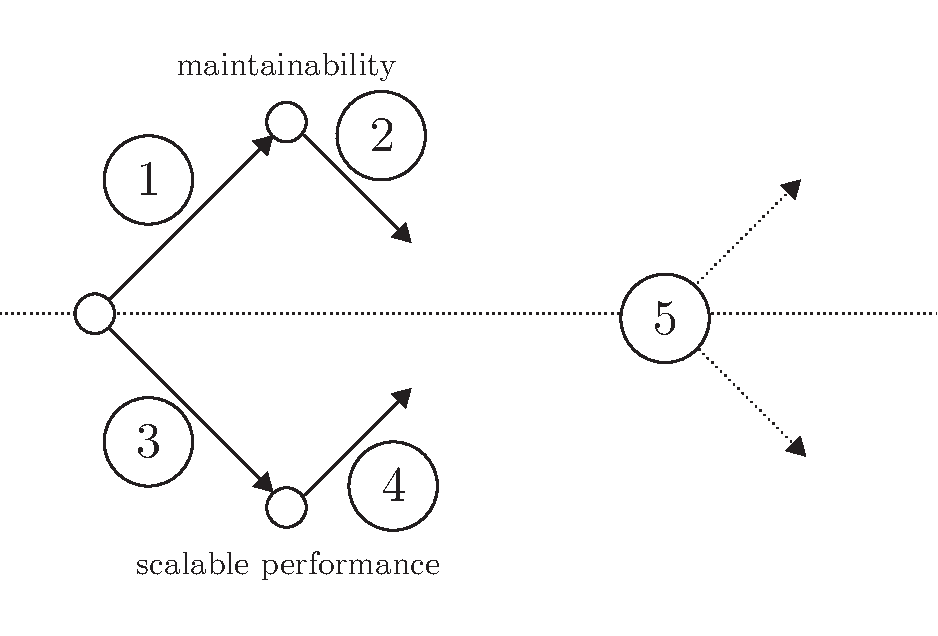
\includegraphics[width=0.6\textwidth]{../ressources/state-of-the-art.pdf}
\end{center}

The evolution of economic constraints often force an SaaS company to switch from scalable development to scalable performance.
This switch implies huge development efforts.
There has been many attempts at reconciling the two goals to reduce these costs.
But none seems really convincing enough to be widely adopted.

The schema above is a graphical representation of the organization of this chapter, and more generally of the state of the art of software design.
The focus on development scalability, noted by number 1, are addressed in section \ref{chapter3:software-maintainability} while the focus on performance scalability, noted by number 3, are addressed in section \ref{chapter3:software-performance}.
Each of these direction of development contains works trying to meet the requirements from the opposing category, noted by number 2 and 4.
And finally, section \ref{chapter3:objectives} presents the objectives for this thesis, noted by number 5.




Present the criteria used for this analysis : 
- higher-order programming, closures, lazy evaluation / stream (not clear)
The expressiveness of a language comes from modularity, which comes from hop and lazy evaluation, because it allows abstraction.
But immutability is difficult, so closures are a good thing too.
So maintainability requires all three.

- shared state (r/w), immutable shared state (r/ø), isolation (ø/ø)
Scalability is about shared state at a fine level, and immutability and isolation at a coarser level.


The state of the art highlights that
\begin{itemize}
\item maintainability requires lazy-evaluation and higher-order programming, section \ref{chapter3:software-maintainability:programming-models:functional-programming}, and
\item higher-order programming requires a global memory abstraction, section \ref{chapter3:software-maintainability:modular-programming:limitations},
\end{itemize}
Javascript is a functional language that features higher-order programming and a global memory abstraction.
% Moreover, its dynamic natures allows a lot of flexibility for the developers.
Moreover, node.js features a streaming approach with the event-loop execution model, similar to the lazy evaluation.
These reasons make Javascript a language of choice for developing web application.

And that
\begin{itemize}
\item scalable performance requires parallelism, and
\item parallelism requires exclusive accesses on the state through isolation and immutability.
\end{itemize}
Eventually, web development is heading toward a streaming approach with pipeline processing.

\nt{TODO dependency schema of these highlights}



These are all the ACADEMIC criteria.

The INDUSTRY criteria are :
- size of the community (to hire, get help, and make things evolve)
- number and fitness of available tools
  ->  web centric


A system is maintainable only if there is competences available to maintain it.

The criteria to analyze the solutions presented in this section regarding the organic growth are : 
\begin{itemize}
\item adoption by the community
\item adoption by the industry
\item supporting web technologies
\end{itemize}
The first two criteria make sure that the technology is growing organically with a passionate community, and backed by industrial needs.
The last criteria assures the fitting of the technologies with our economical context of a web application. 




Maybe take some parts from chapter 2 to put into industry (all the languages comparison stuffs that barely belong in the context).

\section{Software Maintainability} \label{chapter3:software-maintainability}

\cit{It is becoming increasingly important to the data-processing industry to be able to produce more programming systems and produce them with fewer errors, at a faster rate, and in a way that modifications can be accomplished easily and quickly.}{W. P. Stevens, G. J. Myers, L. L. Constantine \cite{Stevens1974}}.

In order to improve and maintain a software system, it is important to holds in mind the mental representation behind its implementation.
Architects, and mechanical engineers draw codified plans to share their mental representations with peers and building teams.
software design is an exception in that the implementation is both the shared mental representation, and the actual product.
The mental representation is often lost in technical details and optimizations for the actual product.
This problem becomes even more critical as the system grows in size.
Therefore, it is crucial to decompose the system into smaller subsystem easier to grasp individually.
This section shows the theories, programming languages and frameworks helping this decomposition.

\subsection{Modular Programming} \label{chapter3:software-maintainability:modular-programming}

The modularity of a software implementation is about enclosing the subproblems and bringing the relevant interfaces to allow these part to be composed.
It allows greater design to emerge from the composition of smaller components.
Such modularity helps organizing the implementation to reflect the underlying mental organization.
The modularity in software design improves the maintainability of an implementation, as presented in the following schema.
It allows to limit the understanding required to contribute to a module \cite{Stevens1974}.
And it reduces development time by allowing several developers to simultaneously implement different modules \cite{Wong2009,Cataldo2006}.

\begin{center}
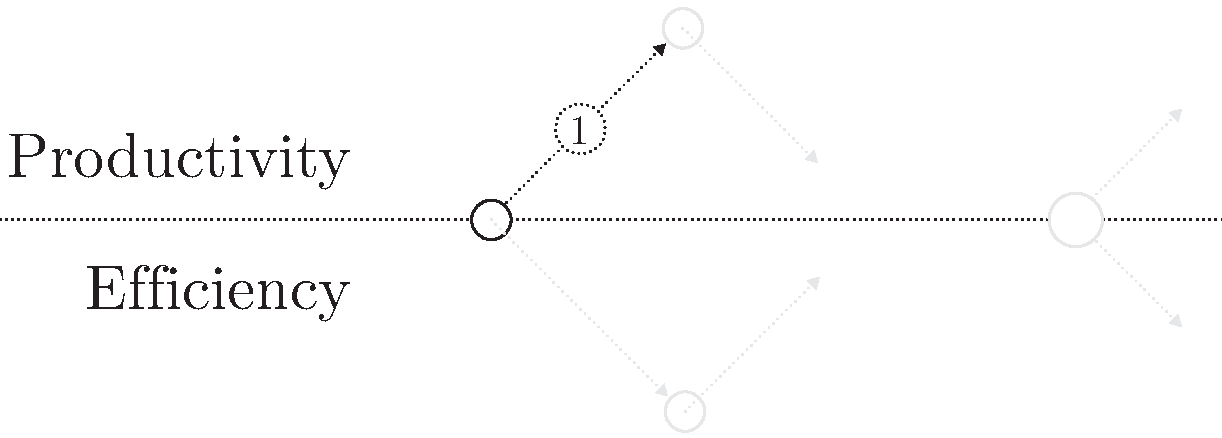
\includegraphics[width=0.6\textwidth]{../ressources/state-of-the-art-1.pdf}
\end{center}

The section \ref{chapter3:software-maintainability:modular-programming:design-choices} is about the decomposition of a problem into subproblems.
Then, the section \ref{chapter3:software-maintainability:modular-programming:programming-models} is about the bringing the interfaces allowing their composition.
Finally, the section \ref{chapter3:software-maintainability:modular-programming:limitations} presents the consequences of this decomposition on performance.


\subsubsection{Design Choices} \label{chapter3:software-maintainability:modular-programming:design-choices}

\nt{TODO this introduction is not very clear}
In the decomposition of a large problem into smaller subproblem, there is two design choices.
The first one is the granularity, and organization of the subproblems within the system decomposition.
The second one is the organization of the implementation within the subproblems to improve maintainability.

\paragraph{System Decomposition}

\illustration{spaghetti programming}

Dijkstra firstly developed the concept of Structured Programming \cite{Dijkstra1970}, which later led to modular programming.
% It is defined as \textit{the systematic use of abstraction to control a mass of details, and also a means of documentation which aids program design} \cite{Knuth1974}.
Structured programming is about drawing clear interfaces around a piece of implementation so that the execution is clearly enclosed inside.
At a fine level, it helps avoid spaghetti code \cite{Dijkstra1968a}, and at a coarser level, it structures the implementation \cite{Dijkstra1968} into modules, or layers.
The next paragraph explains further the criteria to draw the borders around modules.

\illustration{lasagna programming}

\paragraph{Decomposition Criteria}

\nt{move this paragraph closer to OOP ?}
The criteria to decompose the system into well defined modules are coupling and cohesion \cite{Stevens1974}.
The coupling defines the strength of the interdependence between modules, while cohesion defines how strongly the features inside a module are related.
Low coupling between modules and high cohesion inside modules helps logically organize, and understand the implementation.
Hence, it improve its maintainability.
The next paragraph present the approach to build modules helping with the evolution of the implementation.

\paragraph{Development Evolution}

To improve maintainability of implementation, the modular organization should isolate the evolution of a module from impacting the rest of the implementation.
The Information Hiding Principle \cite{Parnas1972}, and the Separation of Concerns \cite{Tarr1999,Hursch1995} are two similar approach to do so.
The information hiding principle advocates to encapsulate a specific design choice in each module.
The Separation of Concerns advocates each module to be responsible for one and only one specific concern.
Examples of separation of concerns are the separation of the form and the content in HTML / CSS, or the OSI model for the network stack.

\subsubsection{Programming Models} \label{chapter3:software-design:programming-models}

The previous section presented the design choices to build modules.
This section presents the programming models providing the interfaces to glue the modules together.
It focus on two main programming models currently used in the industry, object oriented programming and functional programming.

\paragraph{Object Oriented Programming}

\illustration{multiple cells communicating}

Alan Kay, who coined the term, states that Object Oriented Programming (OOP) is about message-passing, encapsulation and late binding.
(There is no academic reference for that, only a public mail exchange\ftnt{http://userpage.fu-berlin.de/~ram/pub/pub\_jf47ht81Ht/doc\_kay\_oop\_en}.)
Message-passing and late binding loosen coupling between objects, while encapsulation is intended to increase cohesion \ftnt{http://williamdurand.fr/2013/06/03/object-calisthenics/}.
% Reducing coupling and increasing cohesion are further sought by object calisthenics, in the chapter 6 of \textit{The Thoughtworks Anthology} \cite{Bay2008}

The very first OOP language was Smalltalk \cite{Goldberg1984}.
It defined the core concept of OOP.
Nowadays, the major emblematic figures of OOP in the software industry are C++ and Java \cite{Gosling2000,Stroustrup1986}.
Though, the trend seems to digress from these languages to evolve toward a more dynamic approach, closer to Functional Programming.
Indeed Javascript adopts some functional features such as dynamic typing and higher-order functions \cite{Ecma1999}.

\paragraph{Functional Programming} \label{chapter3:software-design:programming-models:functional-programming}

% \cit{All problems in computer science can be solved by another level of indirection}{Butler Lampson}

The definition of pure Functional Programming resides in manipulating only mathematical expressions - functions - and forbidding state mutability.
The absence of state mutability makes a function referentially transparent, and thus side-effect free.
The most important pure Functional Programming languages are Scheme \cite{Rees1986}, Miranda \cite{Turner1986}, Haskell \cite{Hudak1992}, Erlang \cite{JoeArmstrong} and Standard ML \cite{Milner1997}.

\nt{TODO find a better argument to say that immutability is unadapted to every day programming}
However, the functional programming concepts are also implemented in other languages along with mutable states.
Major imperative programming languages now commonly present higher-order functions and lazy evaluation to help loosen the couple between modules, define more generic and reusable modules.
\textit{In fine}, it helps developers to write applications that are more maintainable, and favorable to evolution \cite{Hughes1989,Turner1981}.

\paragraph{Higher-Order Programming}
\nt{If possible, include this reference : Continuations and coroutines \cite{Haynes1984}}

Higher-order programming allows to manipulate functions like any other primary value : to store them in variables, or to pass them as arguments.
It replaces the need for most modern object oriented programming design patterns \ftnt{http://stackoverflow.com/a/5797892/933670}.
For example Inversion of Control \cite{Johnson}, the Hollywood Principle \cite{Sweet1985}, and Monads \cite{Wadler1992}.
Higher-order programming help loosen coupling, thus improve maintainability.

In languages allowing mutable state, higher-order functions are implemented as closure, to preserve the lexical scope \cite{Sussman1998}.
A closure is the association of a function and a reference to the lexical context from its creation.
It allows this function to access variable from this context, even when invoked outside the scope of this context.
It eventually tangles the memory references so that it requires a global memory.

\paragraph{Lazy Evaluation}

Lazy evaluation is an evaluation strategy allowing to defer the execution of a function only when its result is needed.
% And according to \cite{Hughes1989}, \textit{Abelson and Sussman stress that streams (lazy list) is a powerful tool for structuring programs \cite{Sussman1983}.
The lazy evaluation of lists is equivalent to a stream with a null-sized buffer, while the opposite, eager evaluation, corresponds to an infinite buffer \cite{VanRoy2003}.
Indeed, the dataflow programming paradigm resulting from lazy lists is particularly adapted for stream processing applications.

The lazy evaluation, as well as streams are powerful tools for structuring modular programs \cite{Sussman1983}.s
Lazy evaluation allows the execution to be organized as a concurrent pipeline, as the stages are executed independently for each element of the stream.
But this concurrency requires immutability of state, or at least isolation of side-effects.
The next section addresses the consequences of higher-order programming and lazy evaluation on parallelism.

% Pipeline parallelism is relevant for multi-pass algorithms \cite{Conway1963}, and it is particularly efficient for stream processing applications.

\subsubsection{Performance Limitations} \ref{chapter3:software-maintainability:modular-programming:limitations}

Functional programming greatly support modularity to improve the maintainability of an application, and its resilience to evolution.
However, the closures introduced by higher-order programming require to share the execution context among modules.
The previous chapter show that sharing makes parallelism difficult.
It is the reason why that maintainability and performance seem hardly compatible.
This section explore in further details the limitation of modular programming regarding performances.

\paragraph{Tighten Memory}

Closures are implemented in languages using a global memory.
And by exchanging closures, two modules intricately share their contexts of execution.
Higher-order programming loosen the couple on the implementation level of the modules, but tighten it on the execution level.
It improves modularity, but it inherently worsens the parallelization hence the performance scalability.

\paragraph{Scalability Limitations}

Parallelizing the execution increases the performances \cite{Amdahl1967,Gunther1993}
But the parallelism is limited because the execution portions sharing state need to be scheduled sequentially.
Hence, to increase the parallelism and performance, the concurrent executions need to be independent, or to coordinate to be scheduled sequentially \cite{Gustafson1988,Gunther1996,Nelson1996,Gunther2002}.
We explain further the reasons of these limitations, and the improvement solutions in the next section.

\paragraph{}

\nt{TODO the transition is not very clear}
The modular organization of implementation is opposed to the organization favoring the parallelization of the execution.
The former organization supports the development scalability, while the latter supports performance scalability.
A program cannot trivially follow an organization that support both development evolution, and performance.
However, D. Parnas advocates the use of an assembler to conciliate the two approaches \cite{Parnas1972}.
The next section shows the improvements for performance and parallelism .
Then, section \ref{chapter3:software-performance} shows the techniques for parallelism.

\subsection{Performance Improvements} \label{chapter3:software-maintainability:performance}

To assure its integrity, the global state of an application imposes the concurrent executions to coordinate their accesses.
This coordination is responsible of the atomicity, and exclusivity of the accesses.
It assures the invariance of the state during its atomic manipulation.
So that developers can group operations in atomic manipulations so as to avoid corruption of the state.

The invariance is assured differently depending on how the state is shared among the concurrent execution.
To increase performance, concurrent executions needs to be as independent as possible to be executed in parallel \ftnt{http://joeduffyblog.com/2010/07/11/thoughts-on-immutability-and-concurrency/}.
% Isolation is independent processes
% Immutability Immutability
% Synchronization is event-loop, multi-thread, lock-free
\begin{description}
  \item[Isolation] If different concurrent executions are commutative \cite{Rinard1996,Clements2013a}, and they share no portion of the state and can be isolated and executed in parallel.
  \item[Immutability] Otherwise, the sharing state portions needs to be immutable to conserve invariance and parallel execution \cite{Gordon2012,Matsakis2012a}.
  \item[Synchronization] If different concurrent executions needs mutation on the state, their accesses are scheduled sequentially.
\end{description}

\begin{center}
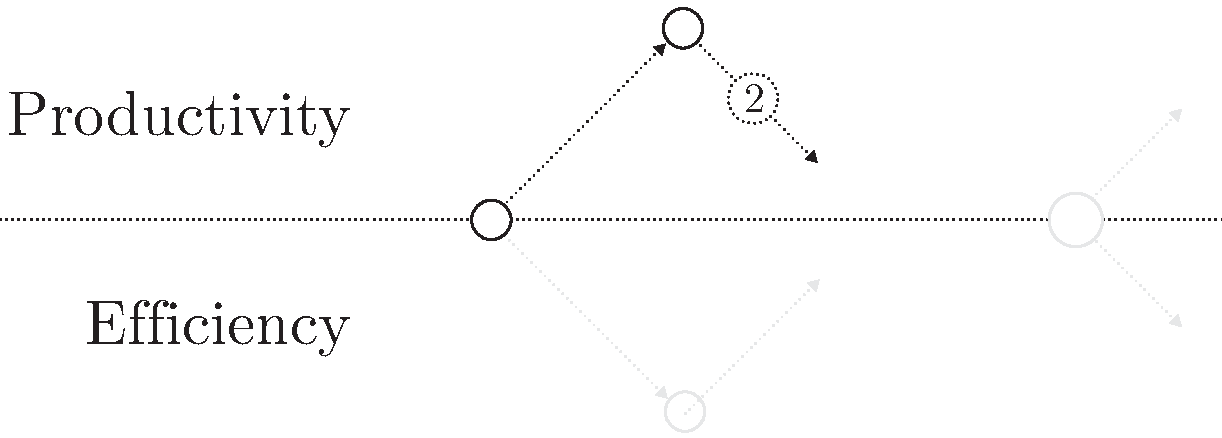
\includegraphics[width=0.6\textwidth]{../ressources/state-of-the-art-2.pdf}
\end{center}

The next few paragraphs presents the different models to assure invariance in concurrent execution, while conserving modular programming, as illustrated in the schema above.
Section \ref{chapter3:software-maintainability:performance:concurrent-programming} presents the programming models providing synchronization and immutability for concurrent executions.
Section \ref{chapter3:software-maintainability:performance:compilation} presents compilation methods to parallelize sequential programs.

% Dynamic Isolation + Making asynchronous parallelism safe for the world \cite{Jr1990}

\subsubsection{Concurrent Programming} \label{chapter3:software-maintainability:performance:concurrent-programming}

% \cit{Building concurrent programming is like building a steam engine through a keyhole}{TODO}

Concurrent programming provides to the developer the mechanisms for concurrent execution, while conserving a global memory model.

\illustration{feu rouge et rond point}

There are two scheduling strategies to execute tasks sequentially on a single processing unit, cooperative scheduling and preemptive scheduling.
Cooperative scheduling allow a concurrent execution to run until it yields back to the scheduler.
Each concurrent execution has an atomic, exclusive access on the memory.
On the other hand, preemptive scheduling allows a limited time of execution for each concurrent execution, before preempting it.
It assures fairness between the tasks, such as in a multi-tasking operating system, but as the preemption happens unexpectedly, the developer needs to lock the shared state to assure atomicity and exclusivity.
The next paragraphs presents the event-based programing model, based on cooperative scheduling, and the multi-threading programming model, based on preemptive scheduling.

\paragraph{Event-Driven Programming}

Event-driven programming explicitly queues the concurrent executions needing access to shared resources.
The concurrent executions are schedule sequentially to assure exclusivity, and cooperatively to assure atomicity.

As presented in the previous chapter, web servers needs to be highly concurrent, and efficient.
The event-driven model is very efficient to serve websites, as it avoids contention due to waiting for shared resources like disks, or network.
Web servers like Flash \cite{Pai1999}, Ninja \cite{Gribble2001} thttpd\ftnt{http://acme.com/software/thttpd/} and Nginx\ftnt{https://www.nginx.com/} were designed following this model.
However, a drawback of this model was that the execution context is lost at each event.
The developer needs to explicitly transfer the relevant state to continue the execution from one event execution to another.

Cooperative threads, or fibers, addressed this drawback \cite{Adya2002,Behren2003a}.
The execution is not ripped into several events.
It yields and resume exactly at the same point after the completion of an asynchronous operation, conserving its context.
However, the developer needs to be well aware of the asynchronous calls to assure the atomicity\ftnt{https://glyph.twistedmatrix.com/2014/02/unyielding.html}.
% + Fibers \cite{Adya2002}
% + Capricio \cite{Behren2003a} - User cooperative threads (also known as fibers / green threads)

The problem of losing the execution context disappears with closures in higher-order programming.
Moreover, the continuation passing style used in higher-order programming requires the developer to be aware of the asynchronous rupture in the execution, so as to assure atomicity \cite{Sussman1998}.
And because an asynchronous call doesn't wait for the completion of the operation, the asynchronous control flow is not limited to be linear like in threads.
Multiple asynchronous calls are made in parallel.
Several execution model proposed this event-based programming model, like TAME \cite{Krohn2007}, Node.js\ftnt{https://nodejs.org/en/} and Vert.X\ftnt{http://vertx.io/}.
% + TAME \cite{Krohn2007} - event-based solution without stack ripping in C (it is like closure, but for C)
% + Node.js - \ftnt{https://nodejs.org/en/}
% + Vert.X - \ftnt{http://vertx.io/} node like + thread / worker capabilities

However, as the shared memory is global and all the execution portions needs atomic access, they are not parallel, but sequentially concurrent.
The next paragraph present the multi-threading and associated synchronization mechanisms to try improve the parallelism of execution using finer granularity of atomic execution and exclusivity.

\paragraph{Multi-Threading Programming}

Threads are light processes sharing the same memory execution context within an isolated process \cite{Dijkstra1968}.
They wait for completion of each operation, and are preemptively scheduled to avoid blocking the global progression.
This preemption breaks the atomicity of the execution, and the parallel execution breaks the exclusivity.
To restore atomicity and exclusivity, hence assure the invariance, multi-threading programming model provide synchronization mechanisms, such as semaphores \cite{Dijkstra}, guarded commands \cite{Dijkstra1975}, guarded region \cite{Hansen1978a} or monitors \cite{Hoare1974}.
They assure an execution region to have exclusive access over a cell of the global state.

\cit{The purpose of explicit synchronization is to manage the timing of side-effects in the presence of parallelism.}{Chris Quenelle\ftnt{http://pchiusano.blogspot.com/2010/01/actors-are-not-good-concurrency-model.html?showComment=1267337235223\#c3014836700278061280}}

Developers tend to use the global memory extensively, and threads require to protect each and every shared memory cell.
This heavy need for synchronization leads to bad performances, and is difficult to develop with \cite{Adya2002}.
The next paragraph present work intending to improve performance by reducing the lock granularity to a minimum.

\paragraph{Lock-Free Data-Structures}

The wait-free and lock-free data-structures reduce the exclusive execution to a few atomic operations \cite{Lamport1977,Herlihy1988,Herlihy1990,Herlihy1991,Anderson1990}.
They are based on transactional memories \cite{Harris2010}, which provide atomic read and write operations on a shared memory.
Lock-free data-structures arrange these atomic operations so as to keep invariance without the need to lock.
They provide concurrent implementation of basic data-structures such as linked list \cite{Valois1995,Timnat2012}, queue \cite{Sundell2003,Wimmer2015}, tree \cite{Ramachandran2015} or stack \cite{Hendler2004}.

However, even if they are theoretically infinitely scalable, they are hard to come with, and are not fit for every problem.

% Reference papers :
% Concurrent reading and writing \cite{Lamport1977}
% Impossibility and universality results for wait-free synchronization \cite{Herlihy1988}
% A methodology for implementing highly concurrent data structures \cite{Herlihy1990}
% Wait-free synchronization \cite{Herlihy1991}

% Book :
% The virtue of Patience: Concurrent Programming With And Without Waiting \cite{Anderson1990}


\paragraph{}

This section section showed that it is difficult for developers to assure the invariance of memory in the context of parallel programming.
Multi-threading programming is inefficient and difficult to program with.
Event-driven programming is easy to develop with but limits parallel execution to assure exclusivity.
The global memory requires the synchronization between concurrent executions to some extent.

Synchronization inherently limits the scalability.
The next section presents compilation methods to improve parallelism, by extracting immutability and isolation from sequential programs.

\subsubsection{Compilation} \label{chapter3:software-maintainability:performance:compilation}

\cit{It is a mistake to attempt high concurrency without help from the compiler}{R. Behren, J. Condit, E. Brewer \cite{Behren2003}}.

When showing the incompatibility between the two organization, D. Parnas  advocated conciliating the two methods using an assembler to transform the development organization into the execution organization \cite{Parnas1972}.
This section presents the state of the art to extract parallelization from sequential programs through code transformation and compilation.

\paragraph{Parallelism Extraction}

As the only requirement to parallelism is the commutativity of operations \cite{Rinard1996,Clements2013a}, a compiler needs to identify the commutative operations transform a sequential program so as to parallelize its execution \cite{Rinard1996}.

An important work was done to parallelize loop iterations \cite{Mauras1989,Amarasinghe1995,Banerjee2013,Radoi2014}, particularly using the polyhedral compilation method \cite{Yuki2013,Grosser2011,Trifunovic2010,Bastoul2004}.
However, this data parallelism is limited to scientific applications because of their heavy use of loops on matrices and vectors.
The performance gains are limited in common sequential programs, as the execution remains sequential outside of loops \cite{Amdahl1967,Clements2013a}.

To improve performance gains further, some compilers identify the data-flow inside sequential programs to allow pipeline parallelism on the whole program, and not only on its loops \cite{Beck1991, Li2012}.
Moreover, the data-flow representation and execution of a program is well suited for modern data processing applications \cite{Fernandez2014a}, as well as web services \cite{Salmito2013}.
\nt{TODO Extract pipeline parallelism compilers from this :
Load balanced pipeline parallelism \cite{Kamruzzaman2013}}

However, the limitation of modular programming regarding parallelization persists.
In a purely functional language with immutability, higher-order functions are referentially transparent which implies commutativity hence parallelism \nt{Add reference of parallel purely functional languages}.
% \cite{Herrmann2000}
However, in a functional language with mutable data, closures remains a challenge to parallelize, because of the memory references shared across the program \cite{Harrison1989, Nicolay2010, Matsakis2012a}.
The next two paragraphs presents two directions to improve the state of the art in parallel compilation.
The first paragraph presents static analysis, while the second presents annotations systems.

% - Continuation-passing style parallelization compilation \cite{Harrison1989}.The interprocedural analysis and automatic parallelization of Scheme programs
% - Automatic Parallelization of Scheme Programs using Static Analysis \cite{Nicolay2010}

% - Commutativity analysis: A new analysis framework for parallelizing compilers \cite{Rinard1996}
% In this paper, they analyze commutative operations to parallelize them.
% It is novel because it isn't about parallelizing loops.
% However, it is not exactly pipeline parallelism either.

% Introducing 'Bones': a parallelizing source-to-source compiler based on algorithmic skeletons \cite{Nugteren2012}

\paragraph{Static analysis}

% Intermediate representation is Abstract Syntax Tree
% Static Single Assignment Form \cite{Cytron1991}
% Continuation Passing Style.

Compilers analyze the control-flow of a program to detect the side-effects causing dependencies between statements \cite{Allen1970}.
The point-to analysis, presented by L. Andersen \cite{Andersen1994} is a popular approach to identify these side-effects in the memory representation.
The points-to-analysis was adapted for Javascript \cite{Jang2009,Sridharan2012,Wei2014}, and is a useful tool to analyze a program.
However, this analysis is not sufficient to track the dynamic control-flow of higher-order functions \cite{Shivers1991} like used in Javascript.

The Operational Semantics is an example of abstract interpretation technique that allows to statically reason on the behavior of programs\cite{Maffeis2008,Smith2011,Gardner2012,Gardner2013,Bodin2014}.
\nt{TODO review this paragraph}
Abstract interpretation techniques are more adapted for program with higher-order functions, and are successfully used for security applications \cite{Huang2004,Jovanovic2006,Yu2007,Maffeis2009a,Chudnov2015,Dolby2015}\nt{Update the citation for Dolby2015}.

However, static analysis techniques are too imprecise, and expensive for the performance gain to be profitable in languages as dynamic as Javascript.
Instead, some compilers relies on annotations from the developers.
% These results suggest that dataflow graphs can serve as an executable intermediate representation in parallel compilers \cite{Beck1991}.

\paragraph{Annotations}

Extracting parallel dataflow from an imperative, sequential implementation is a hard problem \cite{Johnston2004a}.
Some works proposed to rely on annotations from the developer to help the identify the possible side-effects between operations \cite{Vandierendonck2010a,Fernandez2014a}.
% Some works asked the developers to annotate their code so as help the compiler extract parallelism
% It is an intermediate solution with the solution presented in the previous section.

Many compilers rely on annotations from the developer to build highly parallel executables.
Such annotations are especially relevant for accelerators such as GPUs or FPGAs, because the development effort yield huge performance improvements.
Examples of such compilers are OpenMP \cite{Dagum1998}, OpenCL \cite{Stone2010}, CUDA \cite{Nvidia2007} Cg \cite{Mark2003}, Brook \cite{Buck2004}, Liquid Metal \cite{Huang2008}.

However, the burden of detecting commutativity of operations, or independence of operations fall back to the developer.
In this regard, these solutions successfully improve performances, but are unable to fix the rupture between performance and maintainability.
These solutions are indeed very close to the performance oriented solutions presented in the section \ref{chapter3:software-performance}.

% Bloom declarative language \ftnt{http://bloom-lang.net/}
% Blazes: Coordination analysis for distributed programs \cite{Alvaro2014}

% Livescript
% Typescript 
% Annotations, but not for parallelism.
% Asynchronism annotations should be sufficient.

\paragraph{Compilation Limitations}

The static analysis of static, low level languages like FORTRAN or C, brings performance improvements.
However for more dynamic, higher-level languages like Javascript, the static analysis is not sufficient to identify correctly the dependencies between operations to parallelize them.
And parallel compilers often fall back on relying on annotation provided by developers.
So, in this regards, it seems that the accessibility of development gained by higher-level programming is detrimental to performance.

\subsubsection{Accessibility Limitations}

The two previous sections showed that parallel programming is difficult, and that compilation is not yet mature enough to lift this burden from the developer. 

Indeed, preemptive scheduling and synchronization mechanisms are known to be hard to manage by developers, and to impact performances negatively.
On the other hand, cooperative scheduling provides a more accessible invariance abstraction for concurrent programming, but seems limited to sequential execution because of it.

The next section presents the programming paradigms focusing on performance more than development accessibility, and then presents the works to improve accessibility.


% It is easy to understand the parallelism in a cooking recipe because the interdependencies between operations are trivial.
% It seems obvious that melting chocolate is independent from whipping up egg whites.
% % Because chocolate and egg whites are different ingredients.
% This distinction between chocolate and egg whites is trivial.
% % ... comes from the modifications to the state.
% While the distinctions within the state of an application are more intricate.
% This makes concurrent application more difficult to design and implement.





% \paragraph{Transition on parallel programming}

% The definition of separation of concerns given in this section is orthogonal to the original meaning coined by Dijkstra .
% It is interesting to note this difference, as it is related directly to this thesis.
% % Initially, it meant the ability to reason independently about different concern about a software system.
% The initial definition was about analyzing independently how a system meets different concerns.
% Dijkstra gives the example of analyzing independently correctness and efficiency.
% It is impossible to encapsulate correctness, or efficiency in a module, they concern the whole system.
% In this respect, this thesis is oriented towards dissociating the concern of development evolution and of performance.
% That is to be able to reason on the maintainability of a program, independently than of its performance, and vice versa.
% % This seems challenging as D. Parnas opposed these two concerns.
% It is the challenge presented by D. Parnas when he opposed the two concerns in \cite{Parnas1972}.

% This thesis investigates further this opposition to dissociate the concern of evolution and the concern of performance in the case of a web application.
% The next section investigates the first concern, and presents the major programming models used to improve the evolution of an application.

\endinput



remote first Zack Holman : promote asynchronous communication
\ftnt{http://zachholman.com/posts/remote-first/}
+
Conway's law
\cit{Organizations which design systems [...] are constrained to produce designs which are copies of the communication structures of these organizations.}
{M. Conway \cite{Conway1968}}



\subsubsection{Modularity based on Design Decisions}

Designing Software for ease of extension and contraction \cite{Parnas1979}

Design Rules: The Power of Modularity Volume 1 \cite{Baldwin1999}
A reference book, but I can't get it.

Promises 
\cite{Liskov1988}


What makes a great software engineer? \cite{Li2015}

About great software development:
Productivity : Sackman et. al 68, Gugerty & Olson 86
Collaboration, meaningful contribution : Kelly 99, Begel & Simon 06, Hewner & Guzdial 10
Communicate and acquire understanding : LaToza 06, Ko 06
Technical Knowledge : 
Open minded : McConnell 04, Bryant 13



Compiler productivity language into perfomance language
\cite{Kuper2015}\nt{TODO update biblio entry}
\section{Software Performance} \label{chapter3:software-performance}

% The previous section showed that modular programming limits performance scalability of execution.


Moore's law \cite{Moore1965} which forecasts the density of transistors per processing unit, was wrongly interpreted to promise the exponential evolution in the sequential performance of the processing unit, and the assurance for the software industry of always faster hardware.
But as transistors attained a critical size, the reduction in power required by transistor predicted by the Dennard's MOSFET scaling \cite{Dennard2007} stopped\ftnt{https://cartesianproduct.wordpress.com/2013/04/15/the-end-of-dennard-scaling/}.
The ever growing number of transistor predicted by Moore's law are arranged in parallel architecture to continue increasing the performance of processing units.
Parallel programming became the only solution for scalable performance, at the expense of development effort.

This section presents the parallel programming solutions and their limitations in accessibility, and then the improvements to overcome these limitations.

\subsection{Parallel Programming} \label{chapter3:software-performance:parallel-programming}


Concurrent programming is based on the causal ordering of execution.
The ordering of operations is local within a synchronous execution, while the concurrent executions are causally ordered.
It leads to parallel execution with some coordinations such as synchronization, immutability or isolation.
As Lamport showed \cite{Lamport1978}, and Reed related later \cite{Reed2012}, This causal order is sufficient to execute correctly a system in parallel, such as in distributed system.

\begin{center}
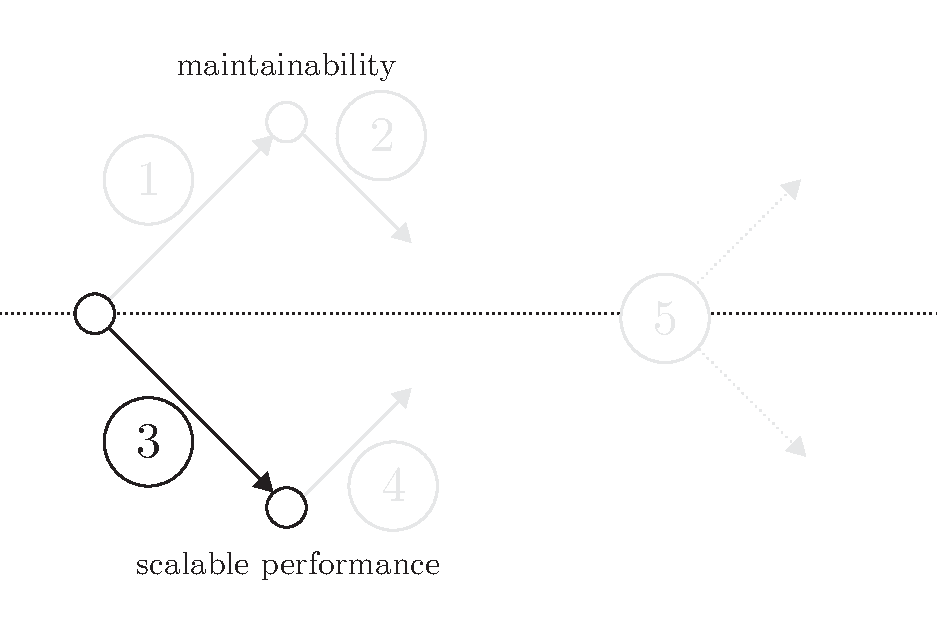
\includegraphics[width=0.6\textwidth]{../ressources/state-of-the-art-3.pdf}
\end{center}

This section presents first hand the theoretical and programming model based on asynchronous communication and isolated execution for parallel programming, as illustrated on the schema above.
It then continues with stream processing programming model. 
And finally,it concludes on the limitations of parallel programming regarding accessibility. 






% All these early work adopted concurrent composition by default, instead of sequential composition, to adapt to the very concurrent nature of real parallel machines.
% However, sequential programming is still the default.
% Concurrent composition is yet still to be widely accepted, as stated by Reed \cite{Reed2012}.
% \comment{TODO rewrite this paragraph}
% \sout{
% % The Actor Model uses asynchronous communications, while $\pi$-calculus uses synchronous communications.
% % Synchronous communications are deterministic.
% % The message sent needs to be received to continue the execution on both ends.
% Because of the synchronous communication used by $\pi$-calculus, the concurrent executions and the communications are both deterministic.
% Therefore, the result of the concurrent system is assured to be deterministic.
% The correctness of the execution of deterministic systems is guaranteed.
% % Determinism is a wanted property to assure the correctness of the execution.
% }

% \sout{
% On the other hand, the asynchronous communications used by Actors are non-deterministic.
% The message sent can take an infinite time to be received.
% Therefore, the result of the concurrent system is not assured to be deterministic.}

% The communication in reality are subject to various faults and attacks \cite{Lamport1982} and too slow compared to execution to be synchronous.

% % And the wait required by synchronous communications negatively impact performances of the system because of the difference of latency between communication, and execution.
% The Actor model was explicitly designed to take these physical limitations in account \cite{Hewitt1977a}.
% The non-determinism in the asynchronous communications is hidden by the organization of the system.
% The total ordering of execution possible with synchronous communication is too strong a requirement for correctness.

% % The non-determinism in the asynchronous communications is hidden by the organization of the system.
% The ordering of execution is only local to an \comment{entity}, while between \comment{entities}, execution is causally ordered.
% The execution will either terminate correctly, or not terminate at all because of a failure in the communications.




% Asynchronous communications are less expressive than synchronous ones \cite{PALAMIDESSI2003}.

% Pi-calculus is a synchronous paradigm which contains an asynchronous fragment.\cite{PALAMIDESSI2003}
% (Boudol, G. (1992). Asynchrony and the π-calculus (note). Rapport de Recherche  1702, INRIA, Sophia-Antipolis,
% Honda, K. and Tokoro, M. (1991).  An object calculus for asynchronous communication. In America, P., editor, Proceedings of the European Conference on Object-Oriented Programming (ECOOP), volume 512 of Lecture Notes in Computer Science, pages 133–147. Springer-Verlag)


% The asynchronous pi-calculus defined by Honda and Tokoro in 1991 led to Pict, a programming language\cite{Pierce2000}.




% There was firstly theories, and models for concurrent computation.
% The main problem was determinism.
% In a sequential machine, the non-determinism of the physical world is hidden by the sequentiality of the machine.
% However, in concurrent computation, the order of communication cannot be assured the way the order of statements is assured in a sequential machine.
% We observe local non-determinism.
% However, to conserve an apparent determinism, causal ordering is sufficient.


\subsubsection{Asynchronous and Isolated Process Parallelism}

The Flynn's taxonomy \cite{Flynn1972} is the most commonly used to categorize parallel execution.
It separates the flow of instructions, and the flow of data ; each being unique, or multiple.
All the current parallel programming model currently belong to the category Multiple Instruction Multiple Data (MIMD), which is further divided into Single Program Multiple Data (SPMD) \cite{Auguin1983,Darema1988,Darema2001} and Multiple Program Multiple Data (MPMD) \cite{Chang1997,Chan2004}.
MIMD implies several threads of execution processing several stream of data.
% The difference between SPMD and MPMD holds on the distinction of instruction pool between the threads of execution.
% SPMD implies to replicate the same program on all the processing units, while MPMD implies to define different programs for every processing units.

% \begin{figure}
% \begin{center}
% 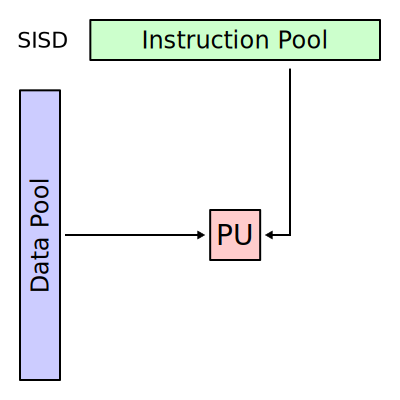
\includegraphics[width=0.2\textwidth]{../ressources/SISD.svg}
% 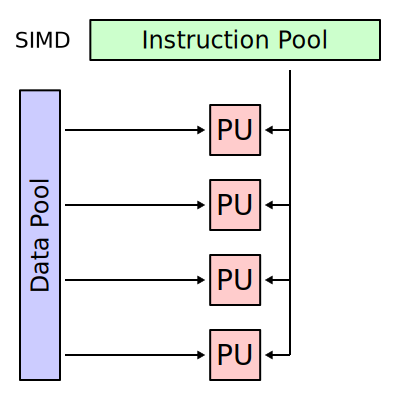
\includegraphics[width=0.2\textwidth]{../ressources/SIMD.svg}
% 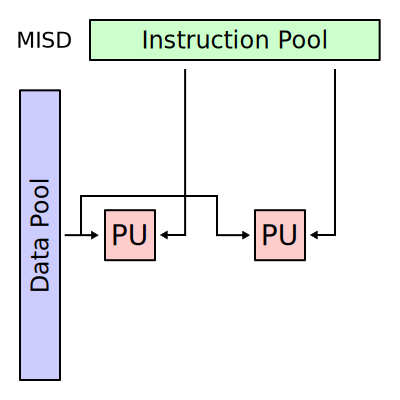
\includegraphics[width=0.2\textwidth]{../ressources/MISD.svg}
% 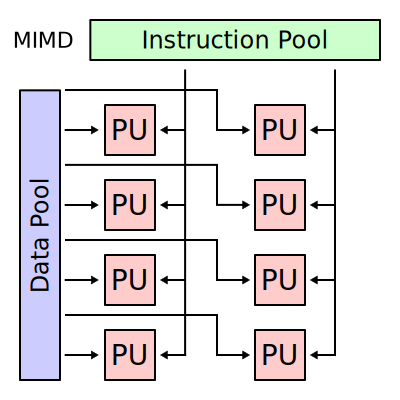
\includegraphics[width=0.2\textwidth]{../ressources/MIMD.svg}\\
% by I, Cburnett. Licensed under CC BY-SA 3.0 via Commons
% \url{https://commons.wikimedia.org/wiki/File:SISD.svg#/media/File:SISD.svg}
% \url{https://commons.wikimedia.org/wiki/File:SIMD.svg#/media/File:SIMD.svg}
% \url{https://commons.wikimedia.org/wiki/File:MISD.svg#/media/File:MISD.svg}
% \url{https://commons.wikimedia.org/wiki/File:MIMD.svg#/media/File:MIMD.svg}
% \end{center}
% \nt{TODO convert these svg to pdf}
% \caption{Flynn's taxonomy of parallelism}
% \end{figure}

\nt{schemas SPMD / MPMD}

The difference between SPMD and MPMD is in the representation of the execution in implementation.
SPMD organizes the implementation as a single execution replicated on many processing units.
While MPMD organizes explicitly the different threads of execution in the implementation.
Examples of SPMD programming languages are
Split-C \cite{Culler},
CRL \cite{Johnson1995} and
Composite C++ \cite{K.ManiChandy2005}.
%
Examples of MPMD programming languages are
Mentat \cite{Grimshaw1991},
Fortran M \cite{Foster1995b} and
Nexus \cite{Foster1996}.
SPMD is close to the model presenting parallel improvements over modular programming presented in section \ref{chapter3:software-design:programming-models}.
While MPMD is closer to the programming models based on isolated process presented in the remaining of this section.
The coordinations between these threads of execution were done by message passing, using PVM \cite{Sunderam1994}, MPI \cite{Snir1996,Walker1996}, SOAP, or the more recent REST protocols.



\paragraph{Theoretical Models}


The communication in reality are subject to various faults and attacks \cite{Lamport1982} and too slow compared to execution to be synchronous.
The Actor model is one of the first programming model to be explicitly designed to take these physical limitations in account \cite{Hewitt1977a}.
It allows to express the computation as a set of communicating actors \cite{Hewitt1973a, Hewitt1977, Clinger1981}.
In reaction to a received message, an actor can create other actors, send messages, and choose how to respond to the next message.
All actors are executed concurrently, and communicate asynchronously.
An asynchronous communication implies that the sender continues its execution immediately after sending the message, before receiving the result of the initiated communication.

In the Actor Model, everything is an actor, even the simplest types like numbers.
This level of granularity is unachievable in practice due to overhead from the asynchronous communications.
Most implementations adopt a granularity on the process or function level.

Coroutines are autonomous programs which communicate with adjacent modules as if they were input and output subroutines \cite{Conway1963}.
It is the first definition of a pipeline to implement multi-pass algorithms.
Similar works include the Communicating Sequential Processes (CSP) \cite{Hoare1978, Brookes1984}, and the Kahn Networks \cite{Kahn1974, Kahn1976}.

% \sout{The first models of computation, like the Turing machine and lambda-calculus, were sequential and based on a global memory state.
% A formalism was missing to represent concurrent computations.
% This section presents the most important works on formalisms for parallel computation.
% They tackled the problems of determinacy, state synchronization and correctness of execution in a formalism based on a network of concurrent processes, asynchronously communicating via messages.
% This section first presents the works on the programming models based on this formalism.
% Then it presents the huge improvements we recently witnessed in the field of distributed stream processing due to the need of performance from the web to process large stream of requests,}

% The mathematical models are a ground for all following work on concurrent programming, we briefly explain them in the next paragraphs.
% There are two main formal models for concurrent computations.
% The Actor Model of C. Hewitt and the Pi-calculus of R. Milner.
% Based on these definitions, we explain the importance of determinism for correctness, and the reasons that made asynchronous message-passing prevail.

% TODO illustration of cells, and draw an analogy between cells and actor model.
% Or something the actor models is based upon.


% The Actor model allows to express the computation as a set of communicating actors \cite{Hewitt1973a, Hewitt1977, Clinger1981}.
% In reaction to a received message, an actor can create other actors, send messages, and choose how to respond to the next message.
% All actors are executed concurrently, and communicate asynchronously.
% The Actor model uses an asynchronous message-passing communication paradigm.
% The communication between two actors, the sender and the receiver, is a stream of discrete messages.
% The sender names the receiver actor when sending messages to be the recipient of these messages.
% An asynchronous communication implies that the sender continues its execution immediately after sending the message, before receiving the result of the initiated communication.

% The Actor model was presented as a highly parallel programming model, but intended for Artificial Intelligence purposes.
% Its success spread way out of this scope, and it became a general reference and influence.
% For example, the Scala programming language features an actor approach to concurrency.

% More recent work of C. Hewitt on Actors is about ... \nt{TODO} \cite{Hewitt2007,Hewitt2007a}.


% R. Milner presented a process calculus to describe concurrent computation : the Calculus of Communicating Systems (CCS) \cite{Milner1975, Milner1980}.
% It is an algebraic notation to express identified processes communicating through synchronous labeled channels.
% % In CCS, process compose concurrently, communications are synchronous, and the topology is static.
% The $\pi$-calculus improved upon this earlier work to allow processes to be communicated as values, hence to become mobile \cite{Engberg1986,Milner1992a,Milner1992}.
% Therefore, similarly to Actors, in Pi-calculus processes can dynamically modify the topology.
% However, contrary to the Actor model, communications in Pi-calculus are based on simultaneous execution of complementary actions, they are synchronous.








% The theory advocates asynchronous message-passing, but it doesn't precise the granularity of the communicating entities.
% In the Actor Model, everything is an actor, even the simplest types, like numbers, similarly in OOP, everything is an object.
% In practice, this level of granularity is unachievable due to overhead from the asynchronous communications.
% Most implementations adopt a granularity on the process or function level.

% % concurrent programming
% The first concept using message passing was the coroutine.
% % It influenced many following works.
% Conway defines coroutines as an autonomous program which communicate with adjacent modules as if they were input and output subroutines \cite{Conway1963}.
% It is the first definition of a pipeline to implement multi-pass algorithms.
% Similar works include the Communicating Sequential Processes (CSP) \cite{Hoare1978, Brookes1984}, and the Kahn Networks \cite{Kahn1974, Kahn1976}.

% Hoare presented the Communicating Sequential Processes (CSP) \cite{Hoare1978, Brookes1984}.
% These processes are executed concurrently, and communicates events via named channels.
% The evolutions of this model were influenced by, and influenced the work of Milner that led to $\pi$-calculus.

% Similarly, Kahn developed the Kahn Networks \cite{Kahn1974, Kahn1976}, following the work of Conway on coroutines.
% They are explicitly parallel coroutines separated by bounded FIFO streams for communication.



% The shared-nothing architecture \cite{Stonebraker1986}.


\paragraph{Programming Languages}

The theoretical models presented above are implemented in industrial languages such as Akka Scala and Erlang.

Scala is an attempt at unifying the object model, and functional programming \cite{Odersky2004}.
% It proposes an actor approach in its design.
Akka\ftnt{http://akka.io/} is a framework based on Scala, following the Actor model to build higly scalable and resilient applications.
Play\ftnt{https://www.playframework.com/} is a web framework based on top of Akka.

Erlang borrow the Actor model as well.
It is a functional concurrent language designed by Ericsson to operate telecommunication devices \cite{JoeArmstrong,Nelson2004} % Nelson2004 is not very good, find another better citation.

\nt{review this paragraph and the transition to the next section}
The field of concurrent programming is so vast it is impossible to relate here every programming languages.
The previous examples are only the best known.
The next focus focuses on streaming real-time applications.

% \comment{transition on lazy evaluation equivalence to stream. lazy evaluation + side effects + concurrency = streams}

\subsubsection{Stream Processing Systems}

All the solutions previously presented are designed to build general distributed systems.
In the context of the web, a real-time application must process high volumes streams of requests within a certain time.
Because these systems are key to business, their reliability and latency are of critical importance.
Otherwise, input data may be lost or output data may lose their value.
These requirements are challenging to meet in the design of such system.

% \textit{
% From a language designer's point of view, real-time
% programs have these characteristics:
% \begin{enumerate}
% \item A real-time program interacts with an environ-
% ment in which many things happen simultaneously at
% high speeds.
% \item A real-time program must respond to a variety
% of nondeterministic requests from its environment. The
% program cannot predict the order in which these requests
% will be made but must respond to them within certain
% time limits. Otherwise, input data may be lost or output
% data may lose their significance.
% \item A real-time program controls a computer with a
% fixed configuration of processors and peripherals and
% performs (in most cases) a fLxed number of concurrent
% tasks in its environment.
% \item A real-time program never terminates but contin-
% ues to serve its environment as long as the computer
% works. (The occasional need to stop a real-time program,
% say at the end of an experiment, can be handled by ad
% hoc mechanisms, such as turning the machine off or
% loading another program into it.)
% \end{enumerate}
% }




\paragraph{Data-stream Management Systems}

% The processing of large volume of data was historically handled by Database management systems.
% These systems naturally evolved to manage data-streams as well.

Database Management Systems (DBMS) historically processed large volume of data, and they naturally evolved into Data-stream Management System (DSMS) to processed data streams as well.
Because of this evolution, they are in rupture with imperative languages presented until now, and borrow the syntax from SQL.

DSMS concurrently run SQL-like requests on continuous data streams.
The computation of these requests spread over a distributed architecture.
Among the early works, we can cite
NiagaraCQ \cite{Chen2000,Naughton2001},
Aurora \cite{Abadi2003,Abadi2003a,Balakrishnan2004} which evolved into
Borealis \cite{Abadi2005},
AQuery \cite{Lerner2003},
STREAM \cite{Arasu2003,Arasu2005} and
TelegraphCQ \cite{Krishnamurthy2003,Chandrasekaran2003}.
More recently, we can cite
DryadLINQ \cite{Isard2007,Yu2009},
Apache Hive \cite{Thusoo2009}\ftnt{https://hive.apache.org/},
Timestream \cite{Qian2013} and
Shark \cite{Xin2013}.


  % + Grape / Timestream - distributed SQL (roughly)
  % + CQL
  % +> STREAM (uses CQL)
  % + StreaQuel
  % +> TelegraphCQ
  % + AQuery

  % + 

% SQL-like
%   AQuery \cite{Lerner2003}
%   STREAM (uses CQL) \cite{Arasu2003,Arasu2005}
%   TelegraphCQ (uses StreaQuel) \cite{Krishnamurthy2003,Chandrasekaran2003}
%   Grape / Timestream - distributed SQL (roughly) \cite{Qian2013}
%   Shark        Stateless dataflow \cite{Xin2013}

%   DryadLINQ    Stateless dataflow \cite{Isard2007,Yu2009}

% \subsubsection{Batched dataflow}

% Map/Reduce
%   MapReduce    Stateless dataflow \cite{Dean2008}
%   Hadoop       Stateless dataflow 
%   Incoop       Incremental dataflow \cite{Bhatotia2011}

% Functional
%   Comet        Batched dataflow \cite{He2010}
%   D-Streams    Batched dataflow \cite{Zaharia2012}
%   Spark        Stateless dataflow \cite{Zaharia,Zaharia2010}
%   Nectar       Incremental dataflow \cite{Gunda2010}





% Imperative Stream Processing
%   Piccolo                                  Parallel in-memory \cite{Power2010}
%   CIEL                                    Stateless dataflow \cite{Murray2011}
%   Statdeful Dataflow Graph (SDG)          Stateful dataflow  \cite{Fernandez2014a}


\paragraph{Pipeline Architecture}

As presented in the previous section, streaming and lazy-evaluation composition both allow a loosely coupled yet efficient composition.
The pipeline architecture takes advantage of this, and composes the parallel execution in a stream, the output of one feeding the input of the next.

SEDA is a precursor in the design of pipeline-based architecture for real-time web applications \cite{Welsh2001}.
It organizes an application as a network of event-driven stages connected by explicit queues.
The event-driven paradigm is similar to previous web servers implementations like Ninja and Flash \cite{Gribble2001,Pai1999}.
SEDA improves with the pipeline organization in stages.

Several projects followed and adapted the principles in this work.
StreaMIT is a language to help the programming of large streaming application \cite{Thies2002}.
Storm \cite{Toshniwal2014} is designed by and used at Twitter to process the heavy streams of tweets.
% It is only one example of industrial practical application, among many others.
Among other works, in the industry, there are
CBP \cite{Logothetis2010} and
S4 \cite{Neumeyer2010}, that were designed at Yahoo,
Millwheel \cite{Akidau2013} designed at Google and
Naiad \cite{Murray2013} designed at Microsoft.

In the litterature, there are
Spidle \cite{Consel2003},
Pig Latin \cite{Olston2008},
Piccolo \cite{Power2010},
Comet \cite{He2010},
Nectar \cite{Gunda2010},
SEEP \cite{Migliavacca2010} and
SDG \cite{Fernandez2014a}

% Similarly to the programming models presented in section \ref{chpater3:concurrent-programming:programming-languages} these frameworks are elitist and not accessible to a large community of developers.
% Indeed, the pipeline architecture presents a distributed storage, which is hardly compatible with the best practices.
% It impacts maintainability.
% For this reason, there are some works on reconciling the concurrent programming models with the modular programming model favoring maintainability.

% + Spidle: A DSL approach to specifying streaming applications dataflow like 


% + Blazes: Coordination analysis for distributed programs \cite{Alvaro2014}



%   (From the paper : Making state explicit for imperative big data processing)
%   + MapReduce       map/reduce   |   Stateless dataflow
%   + DryadLINQ       functional   |   Stateless dataflow
%   + Spark           functional   |   Stateless dataflow
%   + CIEL            imperative   |   Stateless dataflow
%   + Hadoop          map/reduce   |   Stateless dataflow
%   + Incoop          map/reduce   |   Incremental dataflow
%   + Nectar          functional   |   Incremental dataflow
%   + CBP             dataflow     |   Incremental dataflow
%   + Comet           functional   |   Batched dataflow
%   + D-Streams       functional   |   Batched dataflow
%   + Naiad           Dataflow     |   Batched dataflow
%   + Storm, S4       dataflow     |   Continuous dataflow
%   + SEEP            dataflow     |   Continuous dataflow
%   + Piccolo         imperative   |   Parallel in-memory
%   + SDG             imperative   |   Stateful dataflow

%   + pig https://pig.apache.org/
  
% Dataflow
%   CBP          Incremental dataflow \cite{Logothetis2010}
%   S4           Continuous dataflow \cite{Neumeyer2010}
%   Storm        Continuous dataflow \cite{Toshniwal2014}
%   Millwheel    Continuous dataflow \cite{Akidau2013}
%   SEEP         Continuous dataflow \cite{Fernandez2013}
%   Naiad        Batched dataflow \cite{Murray2013}





\comment{Transition on the limitations of software parallelism}

\subsubsection{Elitism of Parallel Programming}

In these parallel programming models describing a network of isolated execution, the topology of the network is statically defined. 
The dynamical modification of the topology is impossible.
It is not possible to dynamically manipulate execution containers, like it is possible to manipulate functions.
Therefore, higher-level programming is impossible, so modular programming is limited.

Moreover, the decomposition of the execution and memory required is difficult for most developers to manage correctly.
\nt{TODO make sure this idea is correctly developed throughout this chapter : parallel programming implies to keep a double mental representation.}
It implies to keep two mental representation of the implementation.
One for the modularity, and one for the decomposition of execution.
Parallel programming remains hard, and is accessible only to an elite of developers.

The next section presents different improvements to make parallel programming more accessible to common developers.





\begin{table}
\small
\begin{tabu} to \linewidth {@{} *1{X[c]} | *2{X[c]} | *1{X[c]} | *2{X[c]} @{}}
%
\toprule
\multicolumn{3}{c}{}  & \multicolumn{1}{|c|}{Concurrency} & \multicolumn{2}{|c}{Parallelism} \\
& Model & Examples    & \multicolumn{1}{|c|}{Synchronization} & Immutability & Isolation \\
\midrule
% ✖ ⨯ ✔                                                                     SYN  IMU  ISO
\multirow{4}{*}{\begin{sideways}\parbox{2.2cm}{Parallel Programming}\end{sideways}} & %
  \multirow{2}{*}{Actor Model}          & Scala, Akka, Play                 & \X & \V & \V \\
&                                       & Erlang                            & \X & \V & \V \\
& \multirow{2}{*}{Stream Processing}    & DSMS (Timestream)                 & \X & \V & \V \\
&                                       & Pipeline (SEDA)                   & \X & \V & \V \\
\bottomrule
\end{tabu}
\caption{Synthesis of the state of the art in parallel programming}
\end{table}














\subsection{Maintainability Improvements} \label{chapter3:software-performance:maintainability}

\comment{Introduction}

As the limitations above state, the difficulties in parallel programming are the absence of higher-level programming, and the decomposition of execution and memory required for parallelism.
This section presents the improvements on accessibility in parallel programing, as illustrated in the schema below.

\begin{center}
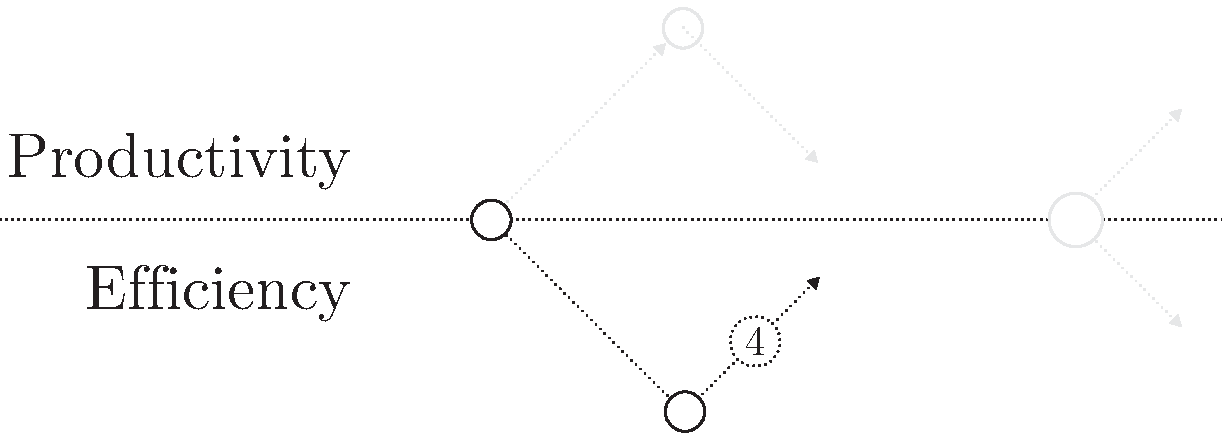
\includegraphics[width=0.6\textwidth]{../ressources/state-of-the-art-4.pdf}
\end{center}

These improvements holds on execution or memory.
This section presents firstly the improvements to ease the decomposition of execution through design patterns and different granularities.
It then presents the improvements to helps development in face of the required memory isolation for distribution.
It then transitions to the lack of improvements for higher-order programming in parallel programing.

\subsubsection{Execution Organization}

All of the parallel programming models presented above decompose the execution into isolated parallel executions, like actors.
This decomposition is difficult as it implies to manage both the parallel decomposition of execution and the modular decomposition of implementation.
Most developers are unable to manage efficiently the two decompositions.
The next paragraphs presents some solutions to mitigate this duality.
\nt{TODO weak argumentation}

\paragraph{Design Patterns}

To reduce the difficulties of the decomposition of the execution into actors, algorithmic skeletons propose predefined patterns that fit certain type of problems \cite{Cole1988, Dean2008, McCool2010, Gonzalez-Velez2010}.
A developer implements the problem as a specific case of a skeleton.
It simplifies the communications, so that the developer can focus on its problem independently of message passing required by the distribution of execution.

% \nt{Link with DSMS}
% As there is similtudes between SQL-like languages, functional structures, and algorithmic skeletons, the latter can be seen as a tentative to merge the more descriptional features of the former into imperative programming.
% Indeed, among the Algorithmic skeletons, we can cite Map / reduce, which are functional structures, but are somehow equivalent to the select and aggregate functions of SQL.
% The pipeline architecture for data stream processing presented in section \ref{chapter3:software-efficiency:dataflow-pipeline} can be considered as algorithmic skeletons.

% However, they introduce limitations and difficulties, as the developer must fit its problem into the skeletons.
% One of this difficulties, it that a common memory is impossible to use.
% Developers needs to think in terms of message passing instead of a global memory, which, as we saw in previous section, is incompatible with best practices.

% Introducing 'Bones': a parallelizing source-to-source compiler based on algorithmic skeletons \cite{Nugteren2012}

\paragraph{Granularity}

The Service Oriented Architectures (SOA), and more recently Microservice\cite{Namiot2014,Fernandez-Villamor2010,Fowler2014,Namiot2014} allow developers to express an application as an assembly of services connected to each others.
Some examples of frameworks are OSGi\ftnt{https://www.osgi.org/developer/specifications/}, EJB\ftnt{http://www.oracle.com/technetwork/java/javaee/ejb/index.html}, Spring\ftnt{http://projects.spring.io/spring-framework/}, and Seneca\ftnt{http://senecajs.org/}
It intends to adjust the granularity of execution decomposition to help developers to fit the two organizations, the modular organization and the parallel execution organization \cite{Adam2008}.

% In modular programming a module protects the rest of the implementation from the consequences of the design choice its encapsulate, while a service encapsulate a specific task, with possible consequences on the adjacent services.

% In a fine enough granularity of service, each service becomes so simple, it can limits the consequences of its modification.

\paragraph{Dynamic Distribution}

An interesting work following SEDA, is Leda \cite{Salmito2013,Salmito2014}.It follows the PCAM design methodology \cite{Foster1995} to propose a model where the stages of the pipeline are defined only by their role in the application.
% Partition $\to$ Communicate $\to$ Agglomerate $\to$ Map.
The actual execution distribution in stages is defined automatically, only after the development, during deployment.
This automation blurs the distinction between the parallel organization of execution, and the modular organization of implementation.
It manages the execution organizations to helps the developer focus on the modular organization.

\paragraph{}

These works helps developers to decompose and distribute the execution of a parallel application.
However, they still propose a distributed memory model.
It doesn't allow higher-level programming, and it requires developers to distribute the state of the application, and assure its isolation.
For these two reason it is difficult to manage.
The next paragraph presents works to improve on the distribution of memory.

% Though, they are still independent, so higher-level programming is impossible.

\subsubsection{Memory Abstraction}

Parallelization of the execution eventually requires the distribution of the memory.
The Partitioned Global Address Space (PGAS) provides the developers with a uniform memory access on a distributed architecture.
It attempts to combine the advantage of SPMD programming style for distributed memory systems, with the data referencing semantics of shared memory systems.
Each computing node executes the same program, and provide its local memory to be shared with all the other nodes.
The PGAS programming model assure the remote accesses and synchronization of memory across nodes, and enforces locality of reference, to reduce the communication overhead.
Examples of implementation of the PGAS model are 
Chapel\cite{Chamberlain2007},
X10 \cite{Charles2005}.
Unified Parallel C \cite{El-Ghazawi2006},
CoArray Fortran \cite{Numrich1998} and
OpenSHMEM \cite{Chapman2010}.

% These programming models are promising.
% However, they focus rather on scientific application with intensive computing such as matrix multiplication, and leave out streaming applications, such as web services.

\paragraph{}

% \nt{TODO PGAS are similar to the programming models presented in the previous section (synchronization).}

The PGAS programming model is similar to the Multi-Threading Programming model presented in section \ref{chapter3:software-maintainability:performance:concurrent-programming}. 
However, it is more focused on performance than modularity.
It focuses on scientific applications with intensive computing such as matrices multiplication.
%, and leave out streaming applications, such as web services.


\subsubsection{Lack of Higher-Order Programming}

% Moreover, 
The programming models of this section lack higher order programming.
% Moreover, in these solutions, higher-order programming is impossible.
As showed earlier in section \ref{chapter3:software-design:programming-models:functional-programming}, higher-order programming is important for modular design and maintainability of the implementation.
In this regards, parallel programming seems currently incompatible with modular programming.
The next section presents the proposition of this thesis to bring parallel programming to a higher-order programming language.
% By keeping the modular programming model, the compilation approach allows higher-level programming.

% \paragraph{Transistion : these methods doesn't allow higher-order programming, which is required for good modularity. WHY ?}

% \nt{TODO link with 3.1}


\begin{table}
\small
\begin{tabu} to \linewidth {@{} *1{X[c]} | *2{X[c]} | *3{X[c]} @{}}
%
\toprule
\multicolumn{3}{c}{} & \multicolumn{3}{|c}{Modularity} \\
& Model & Examples     & Higher-Order Programming & Closures & Lazy Evaluation / Streams \\
\midrule
% ✖ ⨯ ✔                                                                       HOP  CLS  LZY  SYN  IMU  ISO
\multirow{4}{*}{\begin{sideways}\parbox{2.2cm}{Maintainability Improvements}\end{sideways}} & %
  Algorithmic Skeletons                 & Map Reduce ...                    & \X & \X & \V \\
& SOA, Microservices                    & EJB, Spring, Seneca               & \X & \X & \V \\
& Dynamic Distribution                  & LEDA                              & \X & \X & \V \\
& PGAS                                  & Chapel, X10 ...                   & \X & \X & \X \\
\bottomrule
\end{tabu}
\caption{Synthesis of the state of the art in maintainability improvements for parallel programming}
\end{table}













\endinput

\subsection{Concurrency Theory} \label{chapter3:parallel-execution:concurrency-theory}

The mathematical models are a ground for all following work on concurrent programming, we briefly explain them in the next paragraphs.
There are two main formal models for concurrent computations.
The Actor Model of C. Hewitt and the Pi-calculus of R. Milner.
Based on these definitions, we explain the importance of determinism for correctness, and the reasons that made asynchronous message-passing prevail.

% TODO illustration of cells, and draw an analogy between cells and actor model.
% Or something the actor models is based upon.

\subsubsection{Models}

\paragraph{Actor Model}

The Actor model allows to express the computation as a set of communicating actors \cite{Hewitt1973a, Hewitt1977, Clinger1981}.
In reaction to a received message, an actor can create other actors, send messages, and choose how to respond to the next message.
All actors are executed concurrently, and communicate asynchronously.
% The Actor model uses an asynchronous message-passing communication paradigm.
% The communication between two actors, the sender and the receiver, is a stream of discrete messages.
% The sender names the receiver actor when sending messages to be the recipient of these messages.
An asynchronous communication implies that the sender continues its execution immediately after sending the message, before receiving the result of the initiated communication.

The Actor model was presented as a highly parallel programming model, but intended for Artificial Intelligence purposes.
Its success spread way out of this scope, and it became a general reference and influence.
% For example, the Scala programming language features an actor approach to concurrency.

% More recent work of C. Hewitt on Actors is about ... \nt{TODO} \cite{Hewitt2007,Hewitt2007a}.

\paragraph{$\pi$-calculus}

R. Milner presented a process calculus to describe concurrent computation : the Calculus of Communicating Systems (CCS) \cite{Milner1975, Milner1980}.
It is an algebraic notation to express identified processes communicating through synchronous labeled channels.
% In CCS, process compose concurrently, communications are synchronous, and the topology is static.
The $\pi$-calculus improved upon this earlier work to allow processes to be communicated as values, hence to become mobile \cite{Engberg1986,Milner1992a,Milner1992}.
Therefore, similarly to Actors, in Pi-calculus processes can dynamically modify the topology.
However, contrary to the Actor model, communications in Pi-calculus are based on simultaneous execution of complementary actions, they are synchronous.


% Actors can create actors, pi-caclulys processes can replicate, and send processes through channel.
% Processes create a new processes on each instruction to continue the execution.!g systolic arrays

% Pi-calculus resembles to the actor model, but its algebraic nature led to a critical difference with the latter.
% Indeed, processes in the Pi-calculus communicate indirectly, through labeled ports, whereas actors communicate directly by naming the recipient actors.
% This difference allows multiple processes to listen in turns to the same channel, whereas the recipient of a message cannot change.

% I think this difference lead the Pi-calculus to be composable, whereas message-passing is not.
% Message-passing is not composable, whereas invocation is.
% The Actor model is not an ideal programming model, as non-composability makes difficult to reuse or extends existing components.
% A way to compose actors, is to send to an actor the name of the actor to respond to.
% It is similar in essence to the continuation concept.








\section{Reconciliations} \label{chapter3:reconciliations}
\nt{TODO title not clear enough}

\subsection{Contradiction}

The decomposition of an application into a pipeline, as shown in the two previous sections, is incompatible with the modular design advocated by the separation of concerns.
The problem of incompatibility between the modular design and the parallel execution of a pipeline architecture is the following.
There need to be a common understanding on the structure of the communication from one stage to the next.
The modular design defines that this common ground, the interface, be the most resilient possible to focus the evolution within a module.
While the pipeline architecture (and more generally the concurrent programming models) defines these interfaces as the communications between the stages of the execution.
With the evolution of the problem specification, when a stage needs to be modified, it is most likely that these changes will affect the previous or next stages.
% which will eventually change with the evolution of the problem specification.

Most project use languages supporting the modular design at the beginning, when they need to evolve the most.
They then switch to the pipeline architecture only when the requirement of performance overcomes the requirement of evolution.
Moreover, as the team knows that they will eventually throw away their code to upgrade it to a different paradigm, there is little effort to follow the best practice to make maintainable code.
It results in a large effort of development to compensate this rupture.
% This rupture between the two organization is not novel, and is at the center of a large body of work.
In this section, we present the state of the art to reconciliate the two organizations, and avoid this rupture.
First we see the design patterns to fit both organization onto a same source code.
Then we see the compilation tentatives to switch from one to the other.










TO READ :

Flynn's taxonomy
\cite{Flynn1972}

Streaming
\cite{Madsen2015}
\cite{Sun2015}

Map Reduce
\cite{Yao2015}


Web assembly
https://medium.com/javascript-scene/what-is-webassembly-the-dawn-of-a-new-era-61256ec5a8f6
\section{Adoption Focused Platforms} \label{chapter3:software-abstraction}

Section \ref{chapter3:software-maintainability} and section \ref{chapter:software-performance} presented the platforms focusing on maintainability and performance efficiency, and showed that focusing on one negatively impacts the other.
A balance between maintainability and performance efficiency is required to have both the community support and the industrial need, required to be widely adopted.
This section presents platforms featuring an abstraction of the tasks organization to propose a compromise between maintainability and performance efficiency.
Section \ref{chap3:software-abstraction:compilers} presents Compilers, and section \ref{chap3:software-abstraction:runtimes} presents Runtime.

% \nt{read and include \cite{Catanzaro2009} it is about Productivity language JIT compilation into efficient language
% And get all the paper that cite this one.}
% \nt{read and include \cite{Engler1994}}
% \nt{read and include \cite{Kovachev2011}}
% \nt{read and include \cite{Asanovic2006}}

\begin{figure}[!h]
\begin{center}
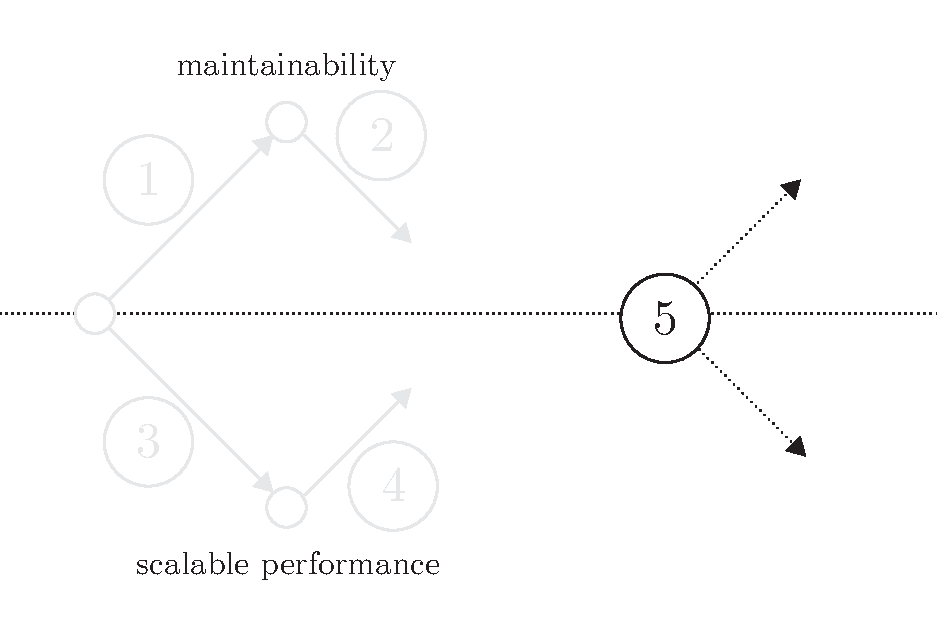
\includegraphics[width=0.6\textwidth]{../ressources/state-of-the-art-5.pdf}
\end{center}
\caption{Focus on Adoption}
\label{fig:state-of-the-art-5}
\end{figure}

\subsection{Abstraction of Tasks Organization}

\subsubsection{Compilers} \label{chapter3:software-abstraction:compilers}

\cit{It is a mistake to attempt high concurrency without help from the compiler}{R. Behren, J. Condit, E. Brewer \cite{Behren2003}}.

As soon as the incompatibility between the modules and the tasks organizations were presented, it was suggested to use a compilation approach to mitigate this incompatibility \cite{Parnas1972}.
% When showing the incompatibility between the two organization, D. Parnas  advocated conciliating the two methods using an assembler to transform the development organization into the execution organization \cite{Parnas1972}.
This section presents the state of the art to extract parallelization from sequential programs through code transformation and compilation.

\nt{read and include \cite{Catanzaro2009}}

\paragraph{Parallelism Extraction}

Extracting parallelism from a sequential implementation is a hard problem \cite{Johnston2004a}.
A compiler needs to identify the commutative operations to parallelize their executions \cite{Rinard1996,Clements2013a}.

An important work was done to parallelize loop iterations \cite{Mauras1989,Amarasinghe1995,Chen2008,Banerjee2013,Radoi2014}, particularly using the polyhedral compilation method \cite{Yuki2013,Grosser2011,Trifunovic2010,Bastoul2004}.
To improve performance gains further, some compilers identify the data-flow inside sequential programs to allow parallelism on the whole program, and not only on its loops \cite{Beck1991,Catanzaro2009,Li2012}.
Moreover, the data-flow representation and execution of a program is well suited for modern data processing applications \cite{Fernandez2014a}, as well as web services \cite{Salmito2013}.
% \nt{TODO Extract parallelism compilers from these :
% Load balanced pipeline parallelism \cite{Kamruzzaman2013}, 
% Regent \cite{Slaughter2015},
% Cilk-P, On-the-Fly Pipeline Parallelism\cite{Lee2013}
% }

% However, the limitation of modular programming regarding parallelization persists.
% In a purely functional language with immutability, higher-order functions are referentially transparent which implies commutativity hence parallelism \nt{Add reference of parallel purely functional languages}.
% \cite{Herrmann2000}
Mutable closures required for higher-order programming remains a challenge to parallelize because of the memory references shared across the program \cite{Harrison1989, Nicolay2010, Matsakis2012a}.
The next paragraphs present some improvements in parallel compilation.
% The first paragraph presents static analysis, while the second presents annotations systems.

% - Continuation-passing style parallelization compilation \cite{Harrison1989}.The interprocedural analysis and automatic parallelization of Scheme programs
% - Automatic Parallelization of Scheme Programs using Static Analysis \cite{Nicolay2010}

% - Commutativity analysis: A new analysis framework for parallelizing compilers \cite{Rinard1996}
% In this paper, they analyze commutative operations to parallelize them.
% It is novel because it isn't about parallelizing loops.
% However, it is not exactly pipeline parallelism either.

% Introducing 'Bones': a parallelizing source-to-source compiler based on algorithmic skeletons \cite{Nugteren2012}

\paragraph{Static analysis}

Compilers statically analyze the control-flow of a program to detect commutative operations \cite{Allen1970}.
The point-to analysis is a popular approach to identify side-effects \cite{Andersen1994,Jang2009,Sridharan2012,Wei2014}.
However, this analysis is not sufficient to track the dynamic control-flow of higher-order functions \cite{Shivers1991} like used in Javascript.

Another approach is the abstract interpretation of the program.
Abstract interpretation techniques are more adapted for dynamic languages like Javascript, and are successfully used for security applications \cite{Huang2004,Jovanovic2006,Yu2007,Maffeis2009a,Chudnov2015,Dolby2015}\nt{Update the citation for Dolby2015}.
It allows to statically reason on the behavior of dynamic program \cite{Maffeis2008,Smith2011,Gardner2012,Hackett2012,Raychev2013,Gardner2013,Bodin2014}.

However, static analysis techniques are too imprecise, and expensive for the performance gain to be profitable.
Instead, some compilers relies on annotations from the developers.

\paragraph{Annotations}

Some works proposed to rely on annotations from the developer to identify the commutativity of operations or the shared data structures \cite{Vandierendonck2010a,Fernandez2014a}.
Such annotations are especially relevant for accelerators such as GPUs or FPGAs, because the development effort yield huge performance improvements \cite{Tarditi2006}.
Examples of such compilers are OpenMP \cite{Dagum1998}, OpenCL \cite{Stone2010}, CUDA \cite{Nvidia2007} Cg \cite{Mark2003}, Brook \cite{Buck2004}, Liquid Metal \cite{Huang2008}.

% Bloom declarative language \ftnt{http://bloom-lang.net/}
% Blazes: Coordination analysis for distributed programs \cite{Alvaro2014}

% Livescript
% Typescript 
% Annotations, but not for parallelism.
% Asynchronism annotations should be sufficient.

\paragraph{Compilation Limitations}

The static analysis of static, low level languages like FORTRAN or C, brings performance improvements.
However for more dynamic, higher-level languages like Javascript, the static analysis is not sufficient to identify correctly the dependencies between operations to parallelize them.
And parallel compilers often fall back on relying on annotation provided by developers.
Hence, the burden of detecting commutativity of operations falls back to the developer, similarly to the platforms presented in the section \ref{chapter3:software-performance}, focusing on performance efficiency.

Alternatively, another approach is to dynamically distribute the commutative operations, and assure the communications.
The next paragraphs present runtime allowing this dynamic distribution.

\subsubsection{Runtimes} \label{chapter3:software-abstraction:runtimes}

\paragraph{Partitioned Global Address Space}

The Partitioned Global Address Space (PGAS) provides the developers with a uniform memory access on a distributed architecture.
It attempts to combine the performance efficiency of distributed memory systems, with the maintainability of shared memory systems.
Each computing node executes the same program, and provide its local memory to be shared with all the other nodes.
The PGAS platform assures the remote accesses and synchronization of memory across nodes.
Examples of implementation of the PGAS model are 
CoArray Fortran \cite{Numrich1998},
X10 \cite{Charles2005}.
Unified Parallel C \cite{El-Ghazawi2006},
Chapel\cite{Chamberlain2007},
OpenSHMEM \cite{Chapman2010}.
Kokko \cite{Edwards2012},
UPC++ \cite{Zheng2014},
RAJA \cite{Hornung2014},
ACPdl \cite{Ajima2015} and
HPX \cite{Kaiser2014,Kaiser2015}


\paragraph{Dynamic Distribution of Execution}

An interesting work following SEDA, is Leda \cite{Salmito2013,Salmito2014}.
% It follows the PCAM design methodology \cite{Foster1995} to 
It proposes a model where the stages of the pipeline are defined only by their role in the application.
% Partition $\to$ Communicate $\to$ Agglomerate $\to$ Map.
The actual execution distribution is defined automatically during deployment. % , only after the development
% blurs the distinction between the parallel organization of execution, and the modular organization of implementation.
This automation manages the execution organizations to help the developer focus on the modular organization.




\paragraph{}

Tables \ref{tab:abstraction-maintainability} and \ref{tab:abstraction-performance} presents the platforms presented in this section regarding maintainability and performance.

\AbstractionMaintainabilityTable{tab:abstraction-maintainability}

\AbstractionPerformanceTable{tab:abstraction-performance}



\subsection{Adoption Limitations}

All the platforms presented in this section come from the need to reduce the development commitment required for performance efficiency.
However, none of these platforms are highly supported by the community because they respond exclusively to industrial needs.

They are limited to scientific applications.

The balance between performance efficiency and maintainability is not sufficient for a community of passionate to gather around the platform.
The platform needs to allow the community to experiment and to start projects.
The context of web development is particularly suited to experiment and start projects.

\AbstractionAdoptionTable{tab:abstraction-performance}

\subsection{Summary}

Table \ref{tab:abstraction-summary} summarizes the characteristics of the platforms presented in this section.

\AbstractionSummaryTable{tab:abstraction-summary}

\endinput
























\section{Due Related works} \label{section:related}

To our knowledge, our work is the first to explore the transformation from continuations to Promises in Javascript, and to state the similarity between Promises and data-flow programming.
This section presents the various works related to ours.
Our work is based on the previous work on Promises and Futures~\cite{Liskov1988}, and their specifications in Javascript\footnote{\url{https://promisesaplus.com/}}\footnote{\url{https://people.mozilla.org/~jorendorff/es6-draft.html\#sec-promise-objects}}.


Because of its dominant position in the web, Javascript is recently subject to a growing interest in the field of static analysis.
We identify two teams working on static analysis for Javascript.
In the Department of Computing, Imperial College London, S. Maffeis, P. Gardner and G. Smith realised a large body of work around the static analysis of Javascript.
Their work is based around an operational semantic~\cite{Maffeis2008} to bring program understanding~\cite{Smith2011,Gardner2012,Gardner2013,Bodin2014}.
Their goal seems to revolve around security applications of this analysis~\cite{Maffeis2009,Maffeis2009a}.
In a collaboration between the programming language research groups at Aarhus University and Universität Freiburg, P. Thiemann, S. Jensen and A. Møller are working on the static analysis of Javascript.
They presented a tool providing type inference using abstract interpretation~\cite{Thiemann2005,Jensen2009,Jensen2012}.
Their goal is to improve the tools available for Javascript developers~\cite{Andreasen}.
Another example of interest for Javascript static analysis is the adaptation of the points-to analysis from L. Andersen's thesis~\cite{Andersen1994} to Javascript, by D. Jang \textit{et al.}~\cite{Jang2009} and S. Wei \textit{et al.}~\cite{Wei2014}.

The industry seems to follow the same trends.
There are some security tools based on static analysis.
We can cite for example, the company Shape Security\footnote{\url{https://shapesecurity.com/}}.
They developed \textit{Esprima}, a Javascript parser, and a serie of tools to help static analysis.
Facebook released flow\footnote{\url{http://flowtype.org/}} on 26 October 2014, a static type checker for Javascript.

Promises combine controls over the execution and the data flow.
It arrange the execution parts sequentialy and assign the result of one into the inputs of the next.
This arrangement seems similar to some works on the field of functional and data-flow programming~\cite{Johnston2004,Cohen2012,Morrison1994,Kahn1974}.
We consider it a first step in the merge of elements from the data-flow paradigm into the imperative paradigm.
The Functional Reactive Programming paradigm pushes the intrication of data and control-flow even further~\cite{Winograd-Cort2013}.

\section{Analysis}

\newgeometry{left=0.5cm, right=0.5cm, top=0.5cm, bottom=0.5cm}
\begin{landscape}
\begin{table}
\small
\begin{tabu} to \linewidth {@{} *2{X[c]} | *2{X[c]} | *3{X[c]} | *1{X[c]} | *2{X[c]} @{}}
%
\toprule
\multicolumn{4}{c}{}    & \multicolumn{3}{|c|}{Modularity}                                  & \multicolumn{1}{|c|}{Concurrency} & \multicolumn{2}{|c}{Parallelism} \\
\multicolumn{2}{c|}{} & Model & Examples    & Higher-Order Programming & Closures & Lazy Evaluation / Streams & \multicolumn{1}{|c|}{Synchronization} & Immutability        & Isolation \\
\midrule
% ✖ ⨯ ✔                                                                       HOP  CLS  LZY  SYN  IMU  ISO
\multirow{2}{*}{\begin{sideways}Section \ref{chapter3:software-maintainability:modular-programming}\end{sideways}} & %
\multirow{2}{*}{\begin{sideways}\parbox{2.3cm}{Modular Programming}\end{sideways}} & %
    Object-Oriented Programming           & C/C++, Java                       & \V & \X & \X & \X & \X & \X \\
& & Functional Programming                & Javascript                        & \V & \V & \V & \X & \X & \X \\
\midrule %
\multirow{5}{*}{\begin{sideways}Section \ref{chapter3:software-maintainability:performance}\end{sideways}} & %
\multirow{5}{*}{\begin{sideways}Concurrent Programming\end{sideways}} & %
    Event-driven                          & Node.js, Vert.X, TAME             & \V & \V & \U & \V & \X & \X \\
& & Multi-Threading                       & Lock, Mutex                       & \U & \U & \U & \V & \X & \X \\
& & Lock-Free Data Structure              &                                   & \U & \U & \U & \V & \X & \X \\
& & \multirow{2}{*}{Compilation}          & Loop parallelization              & \X & \X & \X & \V & \X & \X \\
& &                                       & CUDA, OpenCL, OpenMP ...          & \X & \X & \X & \V & \V & \V \\
\midrule %
\multirow{4}{*}{\begin{sideways}Section \ref{chapter3:software-performance:parallel-programming}\end{sideways}} & %
\multirow{4}{*}{\begin{sideways}\parbox{2.2cm}{Parallel Programming}\end{sideways}} & %
    \multirow{2}{*}{Actor Model}          & Scala, Akka, Play                 & \X & \X & \V & \X & \V & \V \\
& &                                       & Erlang                            & \V & \X & \V & \X & \V & \V \\
& & \multirow{2}{*}{Stream Processing}    & DSMS (Timestream)                 & \X & \X & \V & \X & \V & \V \\
& &                                       & Pipeline (SEDA)                   & \X & \X & \V & \X & \V & \V \\
\midrule %
\multirow{4}{*}{\begin{sideways}Section \ref{chapter3:software-performance:maintainability}\end{sideways}} & %
\multirow{4}{*}{\begin{sideways}\parbox{2.2cm}{Maintainability Improvements}\end{sideways}} & %
    Algorithmic Skeletons                 & Map Reduce ...                    & \X & \X & \V & \X & \V & \V \\
& & SOA, Microservices                    & EJB, Spring, Seneca               & \X & \X & \V & \X & \V & \V \\
& & Dynamic Distribution                  & LEDA                              & \X & \X & \V & \X & \V & \V \\
& & PGAS                                  & Chapel, X10 ...                   & \X & \X & \X & \X & \V & \V \\
\bottomrule
\end{tabu}
\caption{Synthesis of the state of the art in software design}
\end{table}
\end{landscape}
\restoregeometry

TODO

% GOTO chapter 4 - proposition
% \section{Seamless Development} \label{chapter3:objectives}
\nt{TODO title not clear enough}

\begin{center}
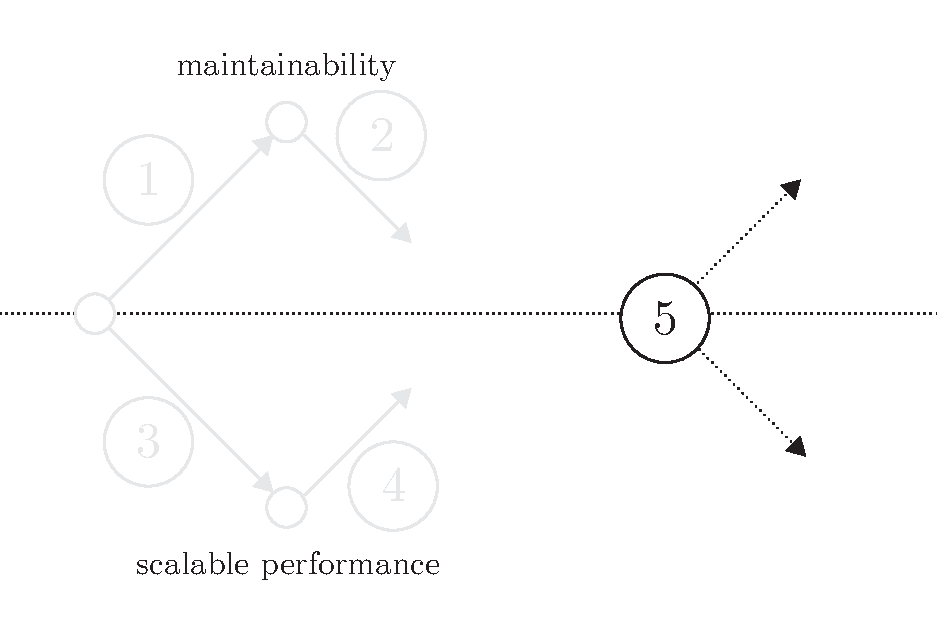
\includegraphics[width=0.6\textwidth]{../ressources/state-of-the-art-5.pdf}
\end{center}

The section \ref{chapter3:software-maintainability} shows that the modular organization enabled by functional programming is the best way to improve maintainability.
But it requires the use of a global memory store which conflicts with performance.
Compilation is a solution to reduce this conflict, but is not yet satisfactory enough for high performance scalability.
On the other hand, the section \ref{chapter3:software-performance} shows that to attain performance scalability, an application needs to multiply the exclusive accesses to its state.
That implies follow a distributed organization of its state to provide isolation and immutability, which negatively impacts modularity, hence maintainability.
Some works provide a uniform memory access to improve maintainability, despite the distributed execution.

The evolution of the economical constraints of a web application requires to repeatedly switch between maintainability and performance scalability.
The incompatibility between the two organizations implies technological ruptures at each switch.
Huge developing efforts are pulled to translate manually from one organization into the other, and later to maintain the implementation despites its unmaintainable nature.
There is still room for improvements on a compromise between maintainability and performance scalability.

The state of the art highlighted that
\begin{itemize}
\item maintainability requires lazy-evaluation and higher-order programming, section \ref{chapter3:software-maintainability:programming-models:functional-programming}, and
\item higher-order programming requires a global memory abstraction, section \ref{chapter3:software-maintainability:modular-programming:limitations},
\end{itemize}
Javascript is a functional language that features higher-order programming and a global memory abstraction.
% Moreover, its dynamic natures allows a lot of flexibility for the developers.
Moreover, node.js features a streaming approach with the event-loop execution model, similar to the lazy evaluation.
These reasons make Javascript a language of choice for developing web application.

And that
\begin{itemize}
\item scalable performance requires parallelism, and
\item parallelism requires exclusive accesses on the state through isolation and immutability.
\end{itemize}
Eventually, web development is heading toward a streaming approach with pipeline processing.

\nt{TODO dependency schema of these highlights}

This thesis proposes an equivalence between the global memory and control flow on one hand, and memory isolation with message passing on the other hand.
It proposes this equivalence as a solution to conciliate the scalable performance and maintainability.
As explained below, the concurrency model of the event-loop execution model, and the parallel approach of the pipeline execution model are very similar.
The goal of this thesis is to allow to compile one execution model into the other, to allow developers to constantly keep two organization of their implementation, allowing them to focus on both maintainability and scalable performance.

\subsection{Equivalence}

The next paragraphs introduces this equivalence between the event-loop execution model and the pipeline execution model.
The equivalence addresses two \textit{levels}\nt{not the good word}, as illustrated in figure \ref{fig:chapter3:objectives:roadmap}, the control flow, and the memory isolation.

\begin{figure}[h!]
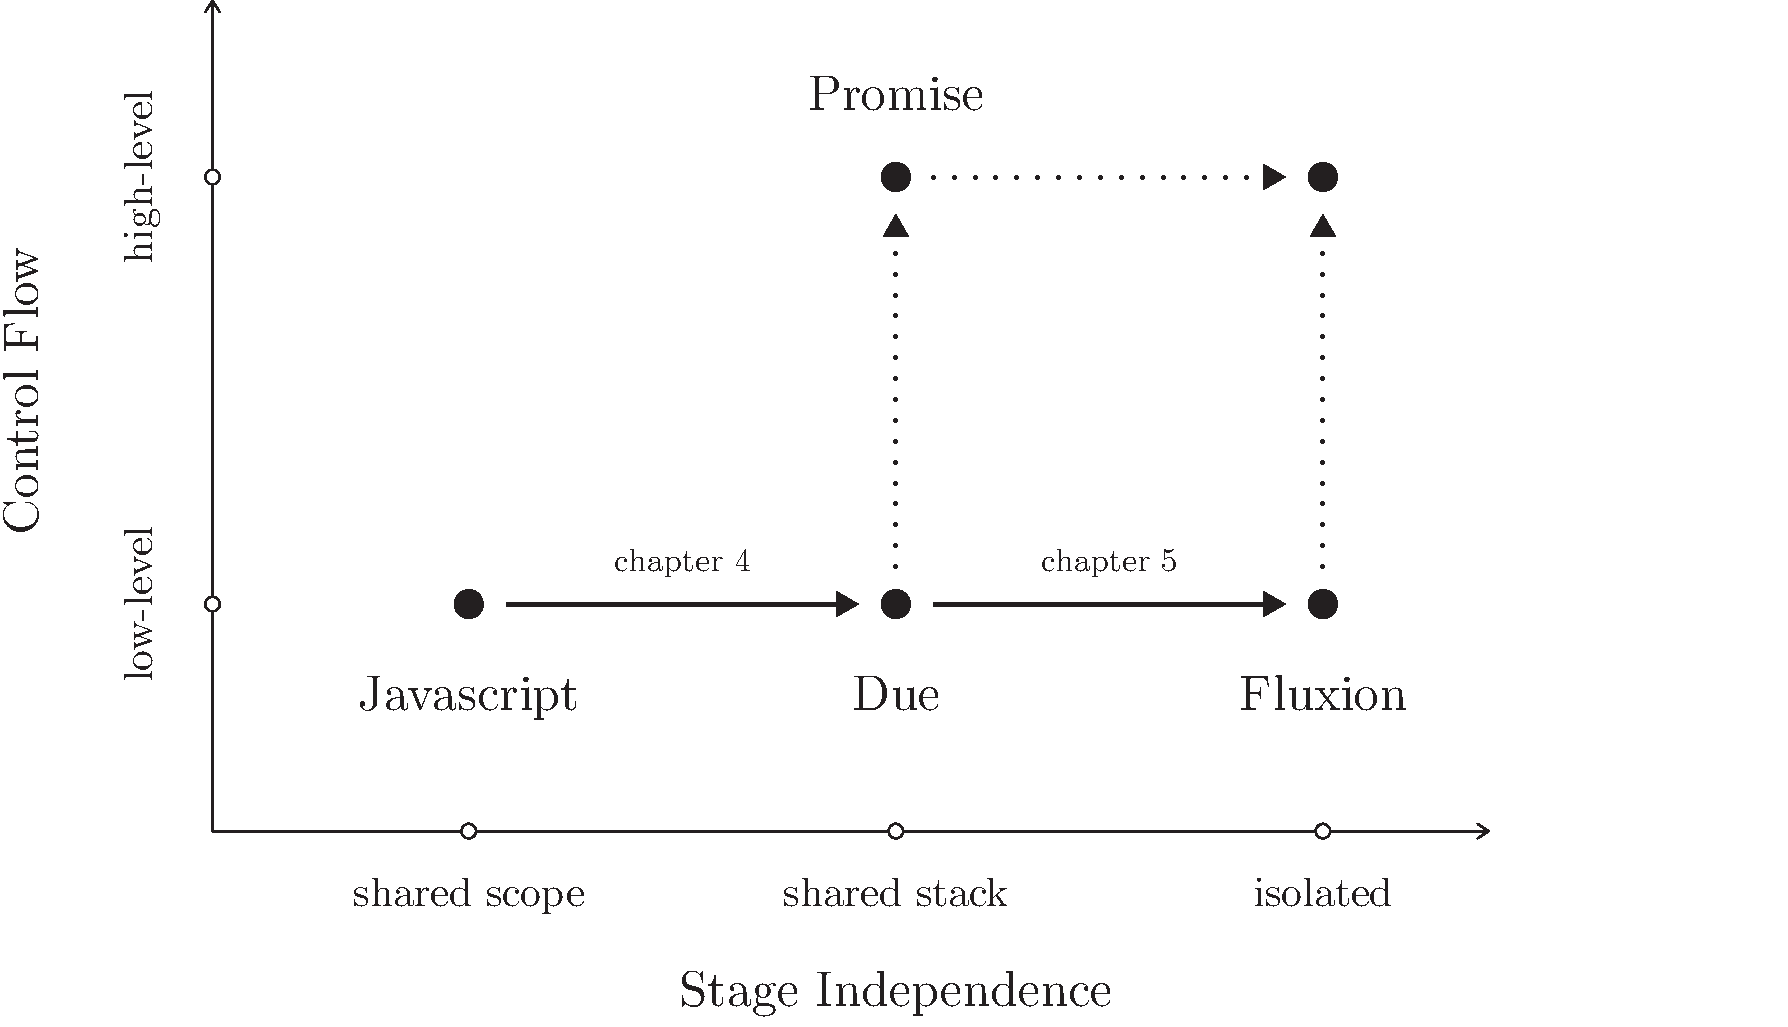
\includegraphics[width=1\textwidth]{../ressources/roadmap.pdf}
\caption{Roadmap}
\label{fig:chapter3:objectives:roadmap}
\end{figure}

\subsubsection{Rupture Point}

The execution of the pipeline architecture is well delimited in isolated stages.
Each stage has its own thread of execution, and is independent from the others.
On the contrary, the code of the event-loop is linear because of the continuation passing style and the common memory store.
% The message passing linking the callbacks is transparently handled by the event-loop.
However, the execution of the different callbacks are as distinct as the execution of the different stages of a pipeline.
The call stacks of two callbacks are distinct.
Therefore, an asynchronous function call represents the rupture between two call stacks.
It is a rupture point, and is equivalent to a data stream between two stages in the pipeline architecture.

Both the pipeline architecture and the event-loop present these rupture points.
The detection of rupture points allows to map a pipeline architecture onto the implementation following the event-loop model.
To allow the transformation from one to the other, this thesis studies the possibility to detect rupture points, and to distribute the global memory into the parts defined by these rupture points.
The detection of rupture points is addressed in chapter \ref{chapter4}.

It presents the extraction of a pipeline of operations from a Javascript application.
Indeed, such pipeline is similar to the one exposed by Promises.
The chapter proposes a simpler alternative to the latter called Dues.
However, these operations still require a global memory for coordination so they are not executed in parallel.

\subsubsection{Invariance}

% This transformation is important on two points.
% The conservation of the invariance.
% The equivalence between the coordinations.

The transformation should preserve the invariance as expressed by the developer to assure the correctness of the execution.
The partial ordering of events in a system, by opposition to total ordering, is sufficient to assure this correctness.
% This result was used by Lamport to prove the correctness of distributed systems.
The global memory is a way to assure the total ordering of events, and the message passing coordination is a way to assure partial ordering of events.
Therefore, to assure the correctness of the execution of a system, the state coordination with a global memory is equivalent to message passing coordination.
And it is possible, at least for some rupture points, to transform the global memory coordination into message passing while conserving the correctness of execution.

In order to preserve the invariance assured by the event-loop model after the transformation, each stage of the pipeline needs to have an exclusive access to memory.
The global memory needs not to be split into parts and distributed into each of the stages.
To assure the missing coordinations assured by the shared memory between the stages, the transformation should provide equivalent coordination with message passing.
The isolation and replacement of the global memory is fully address in chapter \ref{chapter5}, with the introduction of isolated containers called Fluxions.




% The invariance holds for the whole memory during the execution of each callback.
% As I explained in the previous section, this invariance is required to allow the concurrent execution of the different tasks.
% On the other hand, the invariance is explicit in the pipeline architecture, as all the stages have isolated memories.
% The coordination between these isolated process is made explicit by the developer through message passing.

% I argue that the state coordination between the callbacks requireing a global memory could be replaced by the message passing coordination used manually in the pipeline architecture.
% I argue that not all applications need concurrent access on the state, and therefore, need a shared memory.
% % Specifically, I argue that each state region remains roughly local to a stage during its modification.
% \nt{TODO review that, I don't know how to formulate these paragraphs. Identify the state and the data in the global memory.}

% \subsubsection{Transformation}

% This equivalence should allow the transformation of an event loop into several parallel processes communicating by messages.
% In this thesis, I study the static transformation of a program, but the equivalence should also hold for a dynamic transformation.
% I present the analyzis tools I developed to identify the state and the data from the global memory.




%-----------------------------------------------------------------------------%
                                    \endinput
%-----------------------------------------------------------------------------%


Some links I NEED to put :
--------------------------

https://glyph.twistedmatrix.com/2014/02/unyielding.html
http://calculist.org/blog/2011/12/14/why-coroutines-wont-work-on-the-web/

Transitions :
  - Linkedin - http://engineering.linkedin.com/architecture/brief-history-scaling-linkedin
  - Facebook - https://www.cs.princeton.edu/events/event/evolution-software-architecture-facebook / http://www.infoq.com/presentations/Evolution-of-Code-Design-at-Facebook
  - ... 

https://medium.com/@benorama/the-evolution-of-software-architecture-bd6ea674c477

https://en.wikipedia.org/wiki/Dataflow
https://en.wikipedia.org/wiki/Real-time_computing
https://en.wikipedia.org/wiki/Partitioned_global_address_space
https://en.wikipedia.org/wiki/SPMD

Albert Cohen
https://scholar.google.com/citations?user=MkKZKAMAAAAJ&hl=en

+ Paul Feautrier (Tutor of A. Cohen)


Similar problem :
http://2015.splashcon.org/event/splash2015-splash-i-lindsey-kuper-talk
http://www.cs.indiana.edu/~lkuper/papers/lindsey-kuper-dissertation.pdf

PJS was abandoned :
https://groups.google.com/forum/#!topic/mozilla.dev.tech.js-engine/H-YEsejE6DA
https://bugzilla.mozilla.org/show_bug.cgi?id=1117724

See parallel JS for further work (maybe) :
http://smallcultfollowing.com/babysteps/blog/2014/04/24/parallel-pipelines-for-js/

Some chunks I might find useful later :
---------------------------------------

A good example of declarative sentence in everyday world : in case of fire, 
the elevators don't work -> you understand that you need to take the stairs.